% !TEX program = lualatex
\documentclass{matthijs}
\graphicspath{{../assets/}{./docs/assets/}{./docs/technical-design/}}

\begin{filecontents*}[overwrite]{\jobname.xmpdata}
\Title{Technical Design}
\Subject{Implementation description of the lane detection system}
\Author{Matthijs Bakker}
\Language{en-US}
\Keywords{technical\sep design}
\end{filecontents*}

% BEGIN preamble.tex

% Style for first and last page
\usepackage{wallpaper}
\usepackage{color}
\definecolor{arobsblue}{HTML}{0e335c}

% Versioning plugin that retrieves data from the git repo dir
% Needs the "gitInfoHead" file to be generated, make sure
% that the shim script or the git hook is enabled
\usepackage[maxdepth=2]{gitinfo2}

% Use biblatex with biber backend for bibliography
\usepackage{csquotes}
\usepackage[style=ieee]{biblatex}
\renewcommand*{\mkbibacro}[1]{#1}
\setcounter{biburllcpenalty}{7000}
\setcounter{biburlucpenalty}{8000}

% This lets the text look really juicy
\usepackage{microtype}
\usepackage{extdash}

% A column for right-aligned autowrap text
\newcolumntype{R}{>{\arraybackslash}m{10cm}}

% PDF-A
\usepackage{colorprofiles}
\usepackage[a-3b]{pdfx}
\hypersetup{
	bookmarks=true,
	unicode=false,
	pdftoolbar=true,
	pdfmenubar=true,
	colorlinks=true,
	linkcolor=black,
	citecolor=black,
	filecolor=black,
	urlcolor=black
}
%\hypersetup{
%	colorlinks=true,
%	linkcolor=gray,
%	urlcolor=gray,
%	citecolor=gray
%}

% END preamble.tex


\usepackage{titlepage}
\usepackage[title,titletoc]{appendix}

% Load bibliography file
\addbibresource{td.bib}

% Use tikz for drawings
\usepackage{tikz}
\usepackage{tikzscale}
\usepackage{tikz-uml}
\usetikzlibrary{positioning, arrows.meta, matrix}
\usepackage{adjustbox}
\usepackage{pgfplots}
\usepackage{wrapfig}

% Not quite ConTeXt tables but good enough
\usepackage{colortbl}
\usepackage{multirow}
\usepackage{tabularx}

% IEC/ISO units
\usepackage{amsmath}
\usepackage{siunitx}
\sisetup{detect-all}
\sisetup{output-decimal-marker = {,}}
\DeclareSIUnit{\bit}{b}

\begin{document}

	% Set language to English
	\taal{en}

	\maketitlepage{Technical Design}{0.1}
	\pagenumbering{arabic}
	\thispagestyle{empty}

	\begin{inhoudspagina}

		\clearpage

		%\begin{table}[!ht]
			\begin{tabular*}{\textwidth}{l @{\extracolsep{\fill}} R}
				\toprule

				\textbf{Abbreviation} & \textbf{Definition} \\
				\midrule

				ADAS & Advanced Driver-Assistance System \tabularnewline
				ASIC & A non-reconfigurable digital circuit \tabularnewline
				AXIS & AXI Stream; a bus protocol for data streaming interfaces \tabularnewline
				CLB & Configurable Logic Block; the basic physical component of an FPGA fabric that can contain LUTs, FFs and multiplexers. \tabularnewline
				DMA & Direct Memory Access; a way of reading from / writing to memory without utilizing a processor \tabularnewline
				FPGA & Field Programmable Gate Array; a customizable logic circuit \tabularnewline
				Hard-core processor & A dedicated processor as an ASIC \tabularnewline
				HLS & High Level Synthesis; a technique for synthesizing high level computer code to RTL \tabularnewline
				IPI & Vivado IP Integrator; a tool for integrating IP Cores into block designs \tabularnewline
				IP Core & A pre-made digital logic design \tabularnewline
				MPSoC & Multi-Processor SoC; a SoC with multiple physical processing cores; just a marketing term someone at Xilinx made up \tabularnewline
				PL & Programmable Logic; digital logic that can be reconfigured \tabularnewline
				PS & Processing System; everything related to hard- or softcore processors on the device \tabularnewline
				RTL & Register Transfer Level code; a way of describing the behavior of digital logic \tabularnewline
				SoC & System on Chip; a combination of PL and a hard-core processor \tabularnewline
				Soft-core processor & A processor which is implemented in programmable logic \tabularnewline
				VDMA & Video DMA; A DMA controller specially constructed to read/write video data \tabularnewline
				VPU & Vision Processing Unit; refer to chapter 2 of the Functional Design \tabularnewline

				\bottomrule
			\end{tabular*}
			%\label{tabel:Abbreviations}
		%\end{table}

		\vspace{3ex}

		\textbf{Note:} the abbrevation \textit{DRAM} is ambiguous and is often mixed up in FPGA literature.
		In some situations it means \textit{Distributed RAM} (the memory that can be instantiated in SLICEM LUTs~\cite{xilinxug474}) and in other situations it means \textit{Dynamic RAM} (the external memory that is implemented on our FPGA board).
		To avoid confusion, I will be using the abbrevation \textit{SDRAM} to reference the Dynamic RAM variant.

	\end{inhoudspagina}

	\pagenumbering{arabic}
	\tolerance=1
	\emergencystretch=\maxdimen
	\hyphenpenalty=10000
	\hbadness=10000

	\begin{hoofdstuk}{Preface}

		This project is centered around the realization of an ADAS subsystem which can detect the position of a vehicle within a lane.
		A camera is positioned on the dashboard facing the road in front of the vehicle.
		The video feed from this camera is analyzed in real-time by a computer vision system called the Vision Processing Unit.
		This system is implemented on a Field Programmable Gate Array to achieve low-latency detection.
		The output data, existing of information about the lane the car currently occupies, is passed on to the Lane Departure Warning System so that the car can make decisions with it.

		\bigskip

		This document pertains to the technical side of the system.
		The main goal of this document is to give insight on the inner workings of the system so that the knowledge is preserved and modifications to the system can be easily made in the future.
		Design choices and the overcoming of bottlenecks are mentioned to give advice for future projects.
		Another goal is to describe how the system is integrated in a vehicle so that technicians can troubleshoot issues with it.
		The target audience for this document is whom want to get hands-on with the system and its internals.

		\bigskip

		A global system overview is given in the first paragraph to provide context to the reader.
		In the following paragraphs, the layers of the system are described starting with the hardware layer and ending with the software layer.
		The hardware paragraph is about the physical hardware components which are used in the project.
		The programmable logic layer is about the register transfer level code and how it is synthesized on the FPGA.
		The processing system layer is about the program that runs on the processor.
		The software layer is about the troubleshooting software that runs on an external system and can be used by mechanics to see the internals of the processing unit.

		\bigskip

		In this document I will name binary quantities according to the binary multiples convention as described in ISO/IEC 60027-2:2019, which uses the SI prefixes.
		I choose to use this standard because it is widely used in the embedded industry.
		E.g. one kilobit (\qty{1}{\kilo\bit}) is 1000 bits and one kibibit (\qty{1}{\kibi\bit}) is 1024 bits.

	\end{hoofdstuk}

	\begin{hoofdstuk}{System Overview}

		The goal of this paragraph is to describe the problem that the product will solve in different layers of complexity.
		Each layer will dissect the problem into a finer detailed view than the previous.
		This approach gives context to readers who might not be familiar with the fine technical concepts and who wish to grasp the methodology that was used to design the system at a higher level.

		\begin{paragraaf}{Problem Domain}

			Although the system is not directly controlled by a user, many external forces influence the working of the system.
			We have to take them into account when developing the system because they may affect which choices we will make in the development process and how we integrate the system in a vehicle.

			\begin{figuur}{Operational Problem Domain}
				\singlespacing
				\scalebox{0.9}{
					\includegraphics[width=\textwidth]{problem-domain}
				}
				\onehalfspacing
			\end{figuur}

			The system is mainly affected by external forces such as the weather conditions and road quality, which influence the effectiveness of the detection algorithm.
			One such weather condition is water on the road surface.
			It causes refraction of sunlight into the camera lens, which causes the camera to become insensitive to light and the contrast between the road surface and the lane markings to lower.
			The driver of the car influences the detection results by steering the car within the road lane and switching lanes.

		\end{paragraaf}

		\begin{paragraaf}{Information Context}

			The system is connected to different pieces of hardware which all need to communicate with the system to produce an information flow.
			With the diagram in \verwijzingb{figuur}{Information Context Diagram} I want to paint a picture of the general setup of the system.

			\bigskip
			
			The devices are modelled as black boxes because the system does not have access to their internals.
			The only thing known about these devices is that they exchange data via a certain protocol, which the system uses to communicate with them.
			In the later paragraphes of this document, it will be described how the system communicates with these devices.

			\begin{figuur}{Information Context Diagram}
				\singlespacing
				\scalebox{0.9}{
					\includegraphics{information-context-diagram}
				}
				\onehalfspacing
			\end{figuur}
			\vspace{-2ex}

		\end{paragraaf}

		\begin{paragraaf}{Component Definition}

			In order to describe which components make up the total system, I have modeled a SysML Block Definition Diagram.
			This type of diagram shows a black box view of the components that the system consists of.
			It does not represent the inner workings of the system, but rather how it is composed.

			\begin{figuur}{SysML Block Definition Diagram}
				\singlespacing
				\centerline{
					\scalebox{0.75}{
						\includegraphics{block-definition-diagram}
					}
				}
				\onehalfspacing
			\end{figuur}

		\end{paragraaf}

		\begin{paragraaf}{Implementation Strategy}

			Before starting with the implementation phase, I had to figure out in which layer which parts of the system would need to be implemented.
			Different parts of the system have different advantages, e.g. hardware has the potential to have low latency and fast execution and software excels in decision making.
			I explored the capabilities of the PYNQ-Z2 development board and discovered that it has an SoC with an Artix-7 85K programmable logic fabric and a dual-core ARM Cortex A9 processor.
			The processor comes pre-programmed with an embedded Linux distribution that includes the PYNQ platform.
			This PYNQ platform consists of an FPGA programming framework and a Jupyter webserver.
			The programming framework can be used to program pre-generated bitstreams that were created using Vivado onto the FPGA.
			The Jupyter webserver allows the developer to create code snippets -- so-called 'notebooks' -- that run on the embedded Linux distribution and interact with the Programmable Logic via AXI interfaces.
			These AXI interfaces are hard-IP that connect PS and PL with user-definable 32-bit wide digital connections.
		
			\vspace{-0.6ex}
			\begin{figuur}{The Components used for implementing The System}
				\singlespacing
				\includegraphics{implementation-strategy}
				\onehalfspacing
			\end{figuur}
			\vspace{-0.2ex}

			The important concept to understand is that the images which need to be processed are fetched by the Processing System from the capture source.
			I have done this because the connection of a camera is outside the scope of my project and it will be easier to connect the camera to the embedded Linux system because it already has drivers for it.
			Hardware is good at one job, and one job only: the repetetive task it is designed to do, like video processing.
			The results will be delivered back to the PS because it is easier to do business logic like decision making in software.
			This approach also has the benefit of flexibility: software can be modified more quickly than hardware.


		\end{paragraaf}

	\end{hoofdstuk}

	\begin{hoofdstuk}{Integrated Block Design}

		The block design for the system has been created using the Vivado IP Integrator (IPI) because it is the recommended tool to integrate Xilinx IP like the Zynq Processing System in a digital design~\cite{xilinxug994}.
		The design consists of three important components which are connected by diverse utility components.
		These important components are the Zynq Processing System which connects to the hard-core ARMv9 processors, the AXI DMA interface which exchanges memory between PS/PL, and the VPU Image Processing IP Core which is generated by our High Level Synthesis routine.
		The utility components that 'glue' the system in place consist of Xilinx IP Cores like AXI Interconnects that act like buses, AXI Stream Data Width converters that add/remove padding from the video streams and finally the Processor System Reset which manages the reset signals for the interconnects and peripherals.

		\begin{figuur}{Block Diagram of the System Components}
			
			\centerline{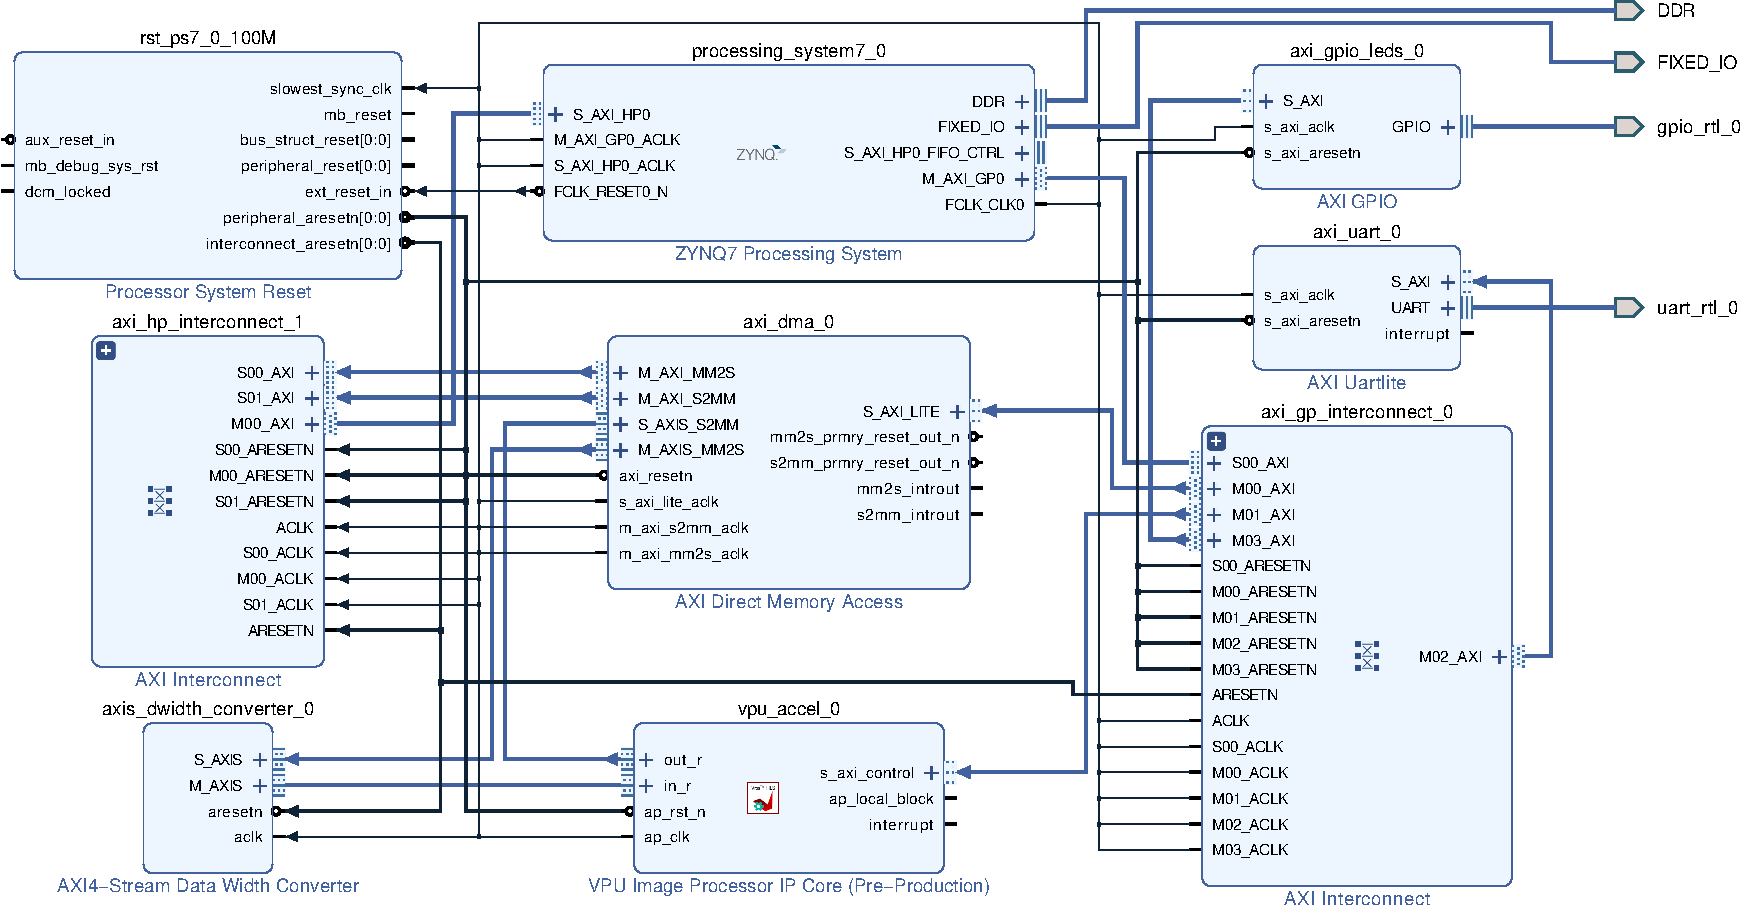
\includegraphics[width=1.2\textwidth]{hw-block-diagram-v2-crop-asset.pdf}}
			
			% "This is a big one and it needs some vspace"
			% -- Sasha Gray, 2022
			\vspace{0.5cm}
			
			(please see \textit{Appendix}\verwijzingn{paragraaf}{Integrated Block Design Diagram}for a magnified version)

		\end{figuur}
		\vspace{-0.35ex} % micro-adjustments to the max

		I've made the decision to only use one global clock net which connects to all components, because I want to prevent components from running off-sync and causing data integrity problems.
		This clock net is derived from the \qty{125}{\mega\hertz} system clock.
		As for the reset signal, I had to create different signals for the interconnects and peripherals because those systems cannot be reset at the same time.
		I used the Processor System Reset component to create these reset signals and I connected the interconnect to the reset ports of the interconnects and data width converters.
		The DMA interface and our Image Processor are connected to the peripheral reset net because these need to be reset after the interconnects are up.

		\bigskip

		The Zynq Processing System has multiple types of hard-IP AXI interfaces, including General Purpose~(GP) interfaces and High Performance~(HP) interfaces.
		Although it would be easy to put every component on the HP interface, this is not the proper way to do it.
		For good measure, I have connected the control interfaces of the DMA and the Image Processor to the GP interface using an interconnect.
		Only the DMA interfaces which need to be low-latency are connected to the HP interface.
		This is done using a dedicated interconnect.

		\bigskip

		Vivado automatically assigned addresses for the components which can be used to access them on the HP AXI and the GP AXI-Lite interfaces.
		I have enabled the generation of a Hardware Handoff (HWH) file, which includes these addresses and automatically passes them on to the PYNQ framework.
		This has the benefit of automatically assigning the addresses to the objects in the Jupyter notebooks, and I won't have to work with the raw addresses.
		If the addresses change or get re-assigned, the HWH file will be automatically regenerated by the Vivado Tcl script and the PYNQ references will be automatically updated.

		\begin{figuur}{Memory Mapped Address Assignments on the AXI Buses}

			\centerline{
				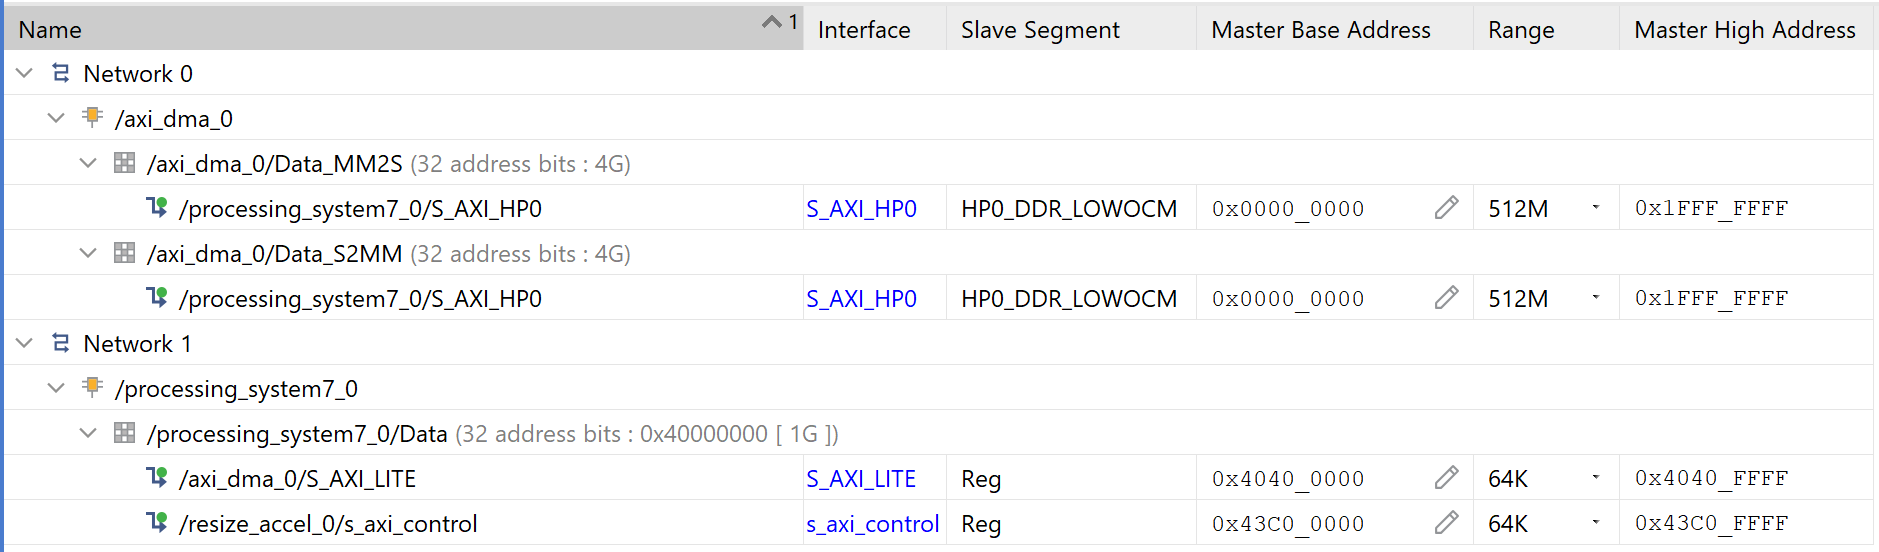
\includegraphics[width=1.1\textwidth, clip, trim=2pt 0 0 2pt]{vivado-bd-address-map-bad-quality.png}
			}

		\end{figuur}
		
		\bigskip

		The DMA is connected to the SDRAM using one of the High Performance AXI ports that comes as hard-IP on the SoC.
		Because the capacity of the SDRAM is half a gibibyte, the range of the memory map has the range to accomodate this.
		It starts at the lowest possible address, 0x0, because the processors expect the system memory to be installed at this location.
		The AXI-HP port has a fixed address size of \qty{32}{\bit}, so this is reflected in the use of the \qty{32}{\bit} addresses for our mapping.
		The DMA is also connected to the Zynq Processing System using an AXI-Lite interface.
		This connection is needed to give control instructions from the software that's running on the PS.

		\bigskip

		Our VPU IP Core is connected to the processing system using AXI-Lite to make the parameters configurable on-the-fly.
		This control interface also provides a way of starting/stopping the video processing function of the core.
		I chose to use an address size of \qty{32}{\bit} to match the size of the hard-IP AXI-GP port that it is connected to.

		\bigskip

		Initially we thought of connecting a camera to the development board to feed the algorithm video data, however, on our new PYNQ board we can simply input images via the framework.
		This change has rendered the camera obsolete, meaning that we don't have to plan I/O pins for it anymore.
		The only pins that are currently used are the hardwired connections and the pre-planned Zynq-PS conections that are retrieved from the board constraints file.
		The package pin planning can be viewed in \verwijzingb{figuur}{FPGA Package Pin Planning}, where orange-marked pins are the pins that are used for the Zynq-PS and connections marked as C or S are hardwired.
		If we wish to use a camera in the future, we have lots of unused pins that could be used to connect it.
		These unused pins are marked with a gray circle on the afforementioned figure.

		\begin{figuur}{FPGA Package Pin Planning}

			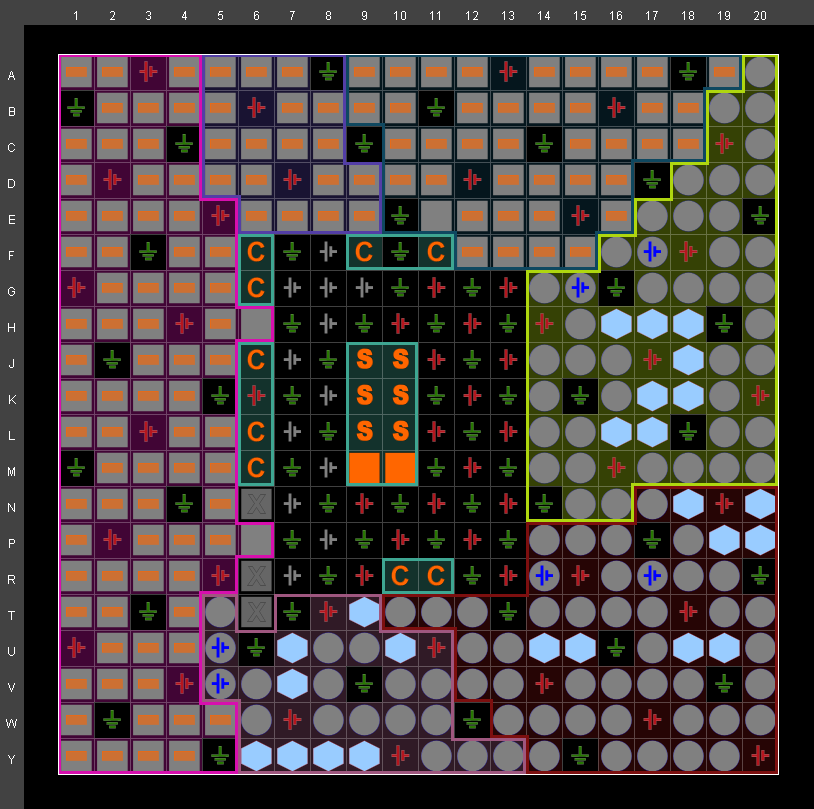
\includegraphics[width=0.8\textwidth]{vivado-synth-package.png}

		\end{figuur}

		Having read up on case studies about high level synthesis, I was worried that we would hit the resource cap because code translation is inherently more inefficient than writing low level code yourself.
		Without creating any timing constraints for the place and route phases, Vivado managed to implement the netlist on the FPGA in an efficient manner.
		It only consumed about 65 percent of the available LUTs and 30 percent of the available FFs while keeping the WNS at \qty{3,2e-11}{\second}, which is 0,3 percent of the clock period. % 0,032 ns :shrug:
		As I talked about in~\verwijzingn{paragraaf}{Memory Configuration}, the BRAM usage is high, but not as high as I expected.
		Due to the proper use of pipelining in the video processing logic, it managed to cram the whole system into only 104 BRAM blocks.
		
		\bigskip

		What I find really interesting is that Vivado has placed the bus infrastructure (AXI interconnects, AXI data width converters, etc) near the Processing System and the VPU IP Core further away from the PS.
		To visualize this in \verwijzingb{figuur}{FPGA Place And Route Floorplan}, I have highlighted with gray color the CLBs that house the bus infrastructure and with yellow color our VPU IP Core.
		This confirms that the place and route phases have been correctly executed and the latency is kept to a minimum.
		It also signals me that I do not need to invest extra time in manually setting timing constraints.

		\vspace{1ex}
		\begin{tabel}{Post-Implementation Utilization Report}{l @{\extracolsep{\fill}} r rr S[table-format=3.1]S[table-format=3.1]}
			\multicolumn{2}{c}{Resource} & \multicolumn{2}{c}{Utilization} & \multicolumn{2}{c}{Utilization \%} \tabularnewline
			\cmidrule{1-2} \cmidrule{3-4} \cmidrule{5-6}
			Type	& Available & \multicolumn{1}{c}{VPU} & \multicolumn{1}{c}{Total}		    & VPU & Total \tabularnewline
			\midrule
			LUT (generic)		& 53200		& 33716 & 36746	& 63.38 & 69.07	\tabularnewline
			LUT (as shift reg)	& 35800		& 276 & 496	& 0.77 & 1.39	\tabularnewline
			LUT (as DRAM)		& 17400		& 48 & 68	& 0.28 & 0.39	\tabularnewline
			FF			& 106400	& 30258 & 34453	& 28.44 & 32.38	\tabularnewline
			DSP			& 220		& 55 & 55	& 25.00 & 25.00	\tabularnewline
			BRAM			& 140		& 99 & 104	& 70.72 & 74.29	\tabularnewline
			BUFG			& 32		& 0 & 1		& 0.00 & 3.13	\tabularnewline

		\end{tabel}

		\begin{figuur}{FPGA Place And Route Floorplan}

			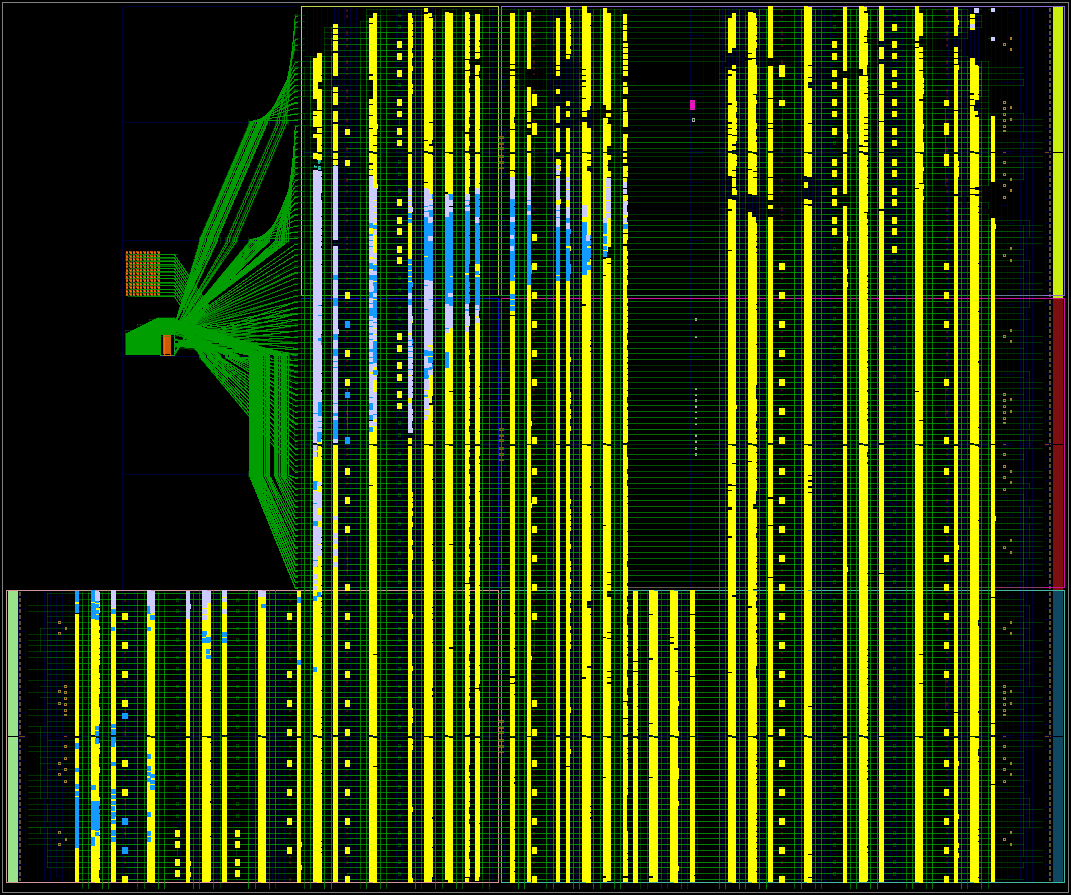
\includegraphics[width=0.8\textwidth]{vivado-impl-placement-full.png}

			\definecolor{floorplanclbwhite}{HTML}{ccccff}
			\definecolor{floorplanclbblue}{HTML}{149bff}
			\definecolor{floorplanclbyellow}{HTML}{ffff00}
			\definecolor{floorplanclbgreen}{HTML}{009e00}

			\vspace{1.5ex}

			\begin{tabular}{rlrl}
				\tikz{\draw[draw=black,fill=floorplanclbwhite] rectangle(1ex, 1ex)} & AXI Bus Infrastructure &
				\tikz{\draw[draw=black,fill=floorplanclbyellow] rectangle(1ex, 1ex)} & VPU IP Core \tabularnewline
				\tikz{\draw[draw=black,fill=floorplanclbblue] rectangle(1ex, 1ex)} & VDMA Controller &
				\tikz{\draw[draw=floorplanclbgreen,line width=0.5mm] (0, 0) -- (1ex, 1ex)} \hspace{-1.325mm} & Connections to PS \tabularnewline
			\end{tabular}

		\end{figuur}

	\end{hoofdstuk}

	\begin{hoofdstuk}{Hardware Layer}

		In this chapter I will describe how and why different hardware components are used in the system.
		The goal is to give a clear picture of the behaviour of the external hardware and which effects it has on the system.

		\begin{paragraaf}{Electrical Schematic}

			The external hardware parts are connected to \textit{board pins} which are exposed on the development board.
			They, in turn, are connected to the FPGA package via so-called \textit{package pins}.
			These package pin names are translated by Vivado to \textit{logical pins} with the use of a constraints file \cite{xilinxug865}.
			In the schematic as seen in \verwijzingb{figuur}{Logical Schematic} I've marked the package pins of the FPGA in red text and the logical pins of my VHDL module in blue text.

			\begin{figuur}{Logical Schematic}
				\centerline{
					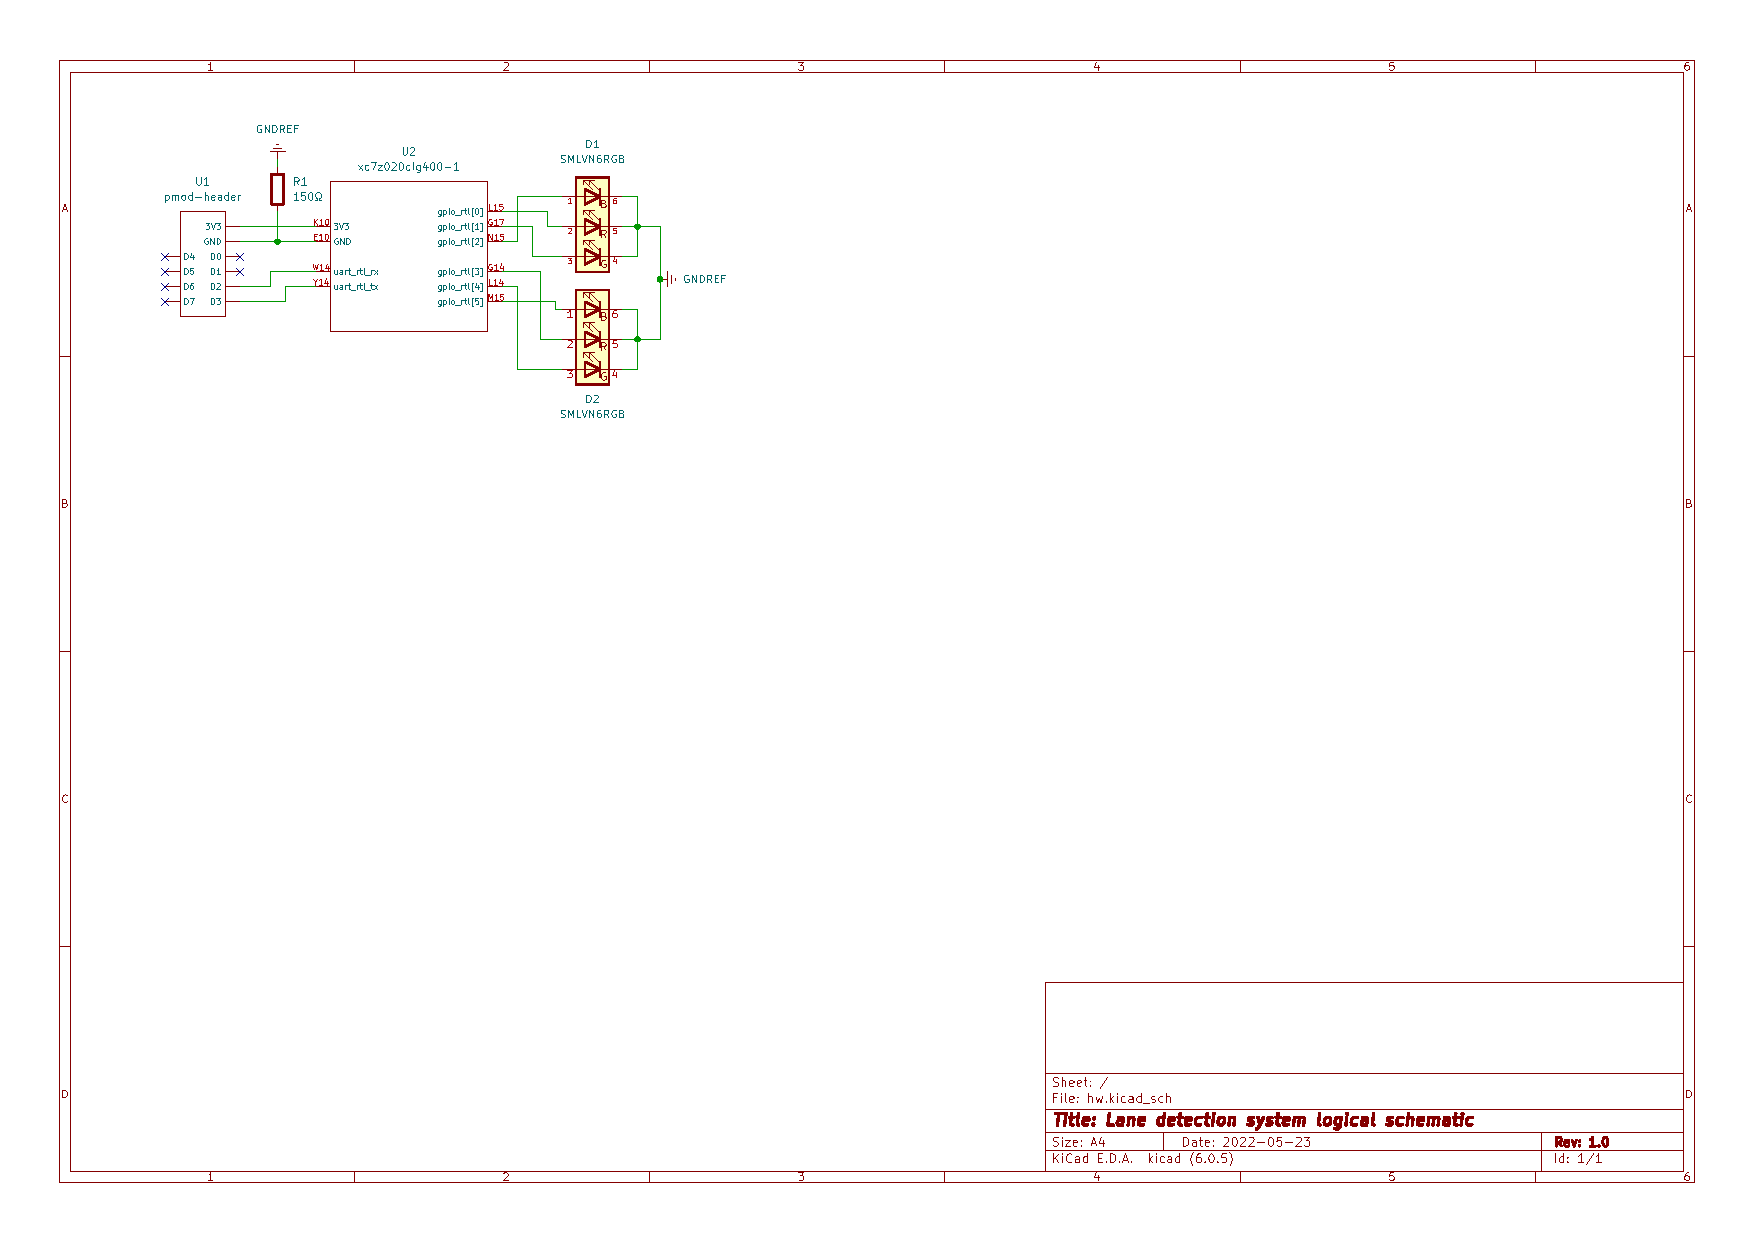
\includegraphics[width=1\textwidth, clip, trim=2.0cm 13.9cm 17.4cm 2.3cm]{hw/hw.pdf/hw.pdf}
				}
				\vspace{-2ex}
			\end{figuur}
			\vspace{-0.8ex}

			The logical output pins of the FPGA are driven at 3.3V to conform with my serial adapter board.
			This voltage is also OK to power the LEDs as noted in the board reference manual~\cite{tul2018pynq}.
			I chose to use the PMOD-B header to place the UART pins because it is mounted on the edge of the board and allows for easy access.
			
			\vspace{0.4ex}
			\begin{figuur}{Setup Picture}
				\centerline{
					\includegraphics[width=0.61\textwidth, clip, trim=7cm 13cm 0cm 22.5cm]{pics/PXL_20220523_101414974.MP.jpg}
				}
			\end{figuur}

		\end{paragraaf}

		\clearpage

		\begin{paragraaf}{Memory Configuration}

			With the initial development board, the Arty A7-35T, I faced a problem regarding the storage of the video frames.
			It had to do with the limited amount of Block RAM (BRAM) on the FPGA.
			The camera outputs an image of 640 by 480 pixels with a configurable color channel configuration of RGB444, RGB555 or RGB565.
			We prefer to have the highest color depth due to the image processing algorithm working better if there is more input variance.
			The FPGA on the Arty board only had \qty{1800}{\kibi\bit} of BRAM, which was not enough to store a full image frame of the lowest color configuration, as can be seen in \verwijzingb{tabel}{Required space to store images of different sizes}.
			One technique to fit the image into memory is to downscale it, but we would lose information on image features which would have an impact on the quality of detection.

			\begin{tabel}{Required space to store images of different sizes}{l @{\extracolsep{\fill}} r r}
				\emph{Bits per channel (BPC)} & 640$\times$420 px & 320$\times$240 px \tabularnewline
				\midrule
				4+4+4 = 12 b & 3150 Kib & 900 Kib \tabularnewline
				5+5+5 = 15 b & 4500 Kib & 1125 Kib \tabularnewline
				5+6+5 = 16 b & 4800 Kib & 1200 Kib  \tabularnewline
			\end{tabel}
			
			The alternatives places to store an image were the \qty{16}{\mebi\byte} of Quad-SPI flash or the \qty{256}{\mega\byte} DDR3L SDRAM.
			The QSPI flash memory had two downsides: it required controller logic which is only available as an IP Core with a full AXI4 bus, making it difficult to use, and it would have been shared with the MicroBlaze flash sector, so we would have had to make sure not to overwrite those contents.
			The DDR3L SDRAM had one major downside: it required the use of the proprietary Xilinx Memory Interface Generator (MIG) which Digilent does not provide any support for.
			The MIG provides little to no abstraction over the raw DDR3 protocol, making it a challenge of its own to implement it.
			Besides, it is a soft IP, which means that it is delivered in a generic way and the developer has to tailor it to the specific board.
			What makes the SDRAM appealing is its high input clock speed of \qty{166}{\mega\hertz} and the ability to read/write \qty{128}{\bit} of information per cycle.
			This high data throughput would mean that we would not have to worry about speed limitations.
			However, the trade-off between the complexity of implementing the memory interface and the benefits that it would bring would need to be considered.

			\bigskip

			The problems with the memory on the Arty A7 development board as I described above made me question the choice of using this particular board.
			I reevaluated the choice and started exploring other development boards.
			Along the way, I discovered the Zynq-7000 SoC lineup that is officially supported by the Vitis Vision libraries.
			One of the cheapest boards available that has a Zynq-7000 SoC is the TUL PYNQ-Z2.
			The SoC on this development board provides a predefined AXI interconnect between the PL and PS which connects the SDRAM via AXI buses.
			In the PL, this SDRAM can be accessed using a hard IP VDMA controller which provides data over AXI Stream buses.
			These AXI Stream buses can be connected to those on the the Vitis Vision HLS-generated RTL solution.
			Another reason why I chose the PYNQ-Z2 is its larger BRAM capacity; it has \qty{4900}{\kibi\bit} of BRAM.
			However, if using the PYNQ Processing System, this memory will be shared with the processor component, leaving a smaller usable space.
			My final decision is to use the DDR3 SDRAM because it is plentyful on the Z2 board: all \qty{512}{\mega\byte} is available to the developer.

			\bigskip

			The final memory optimization I want to talk about is the use of buffering inside the video processing logic.
			For many image operations (especially those that use convolution, like a simple median filter or the Sobel filter) only a small region of the image is needed for computation at a time.
			Let's think of a simple 3x3 median filter: for each pixel it needs the eight neighbouring pixels to determine the resulting color value.
			To process a row of an image, we would only need to load the pixels of the rows above and below the target row.
			Such a row of pixels is frequently called a "line buffer."
			By using this technique of only loading the pixels that we need to do a regional computation, we do not have to load the entire image into memory and thus we can make way with a smaller amount of memory \cite{hoorick2019convolution}.
			The region that the median kernel operates upon is called a "window."
			In \verwijzingb{figuur}{Line buffering and sliding windows} we can see how the line buffers are used for the image operation.
			
			\begin{figuur}{Line buffering and sliding windows}
				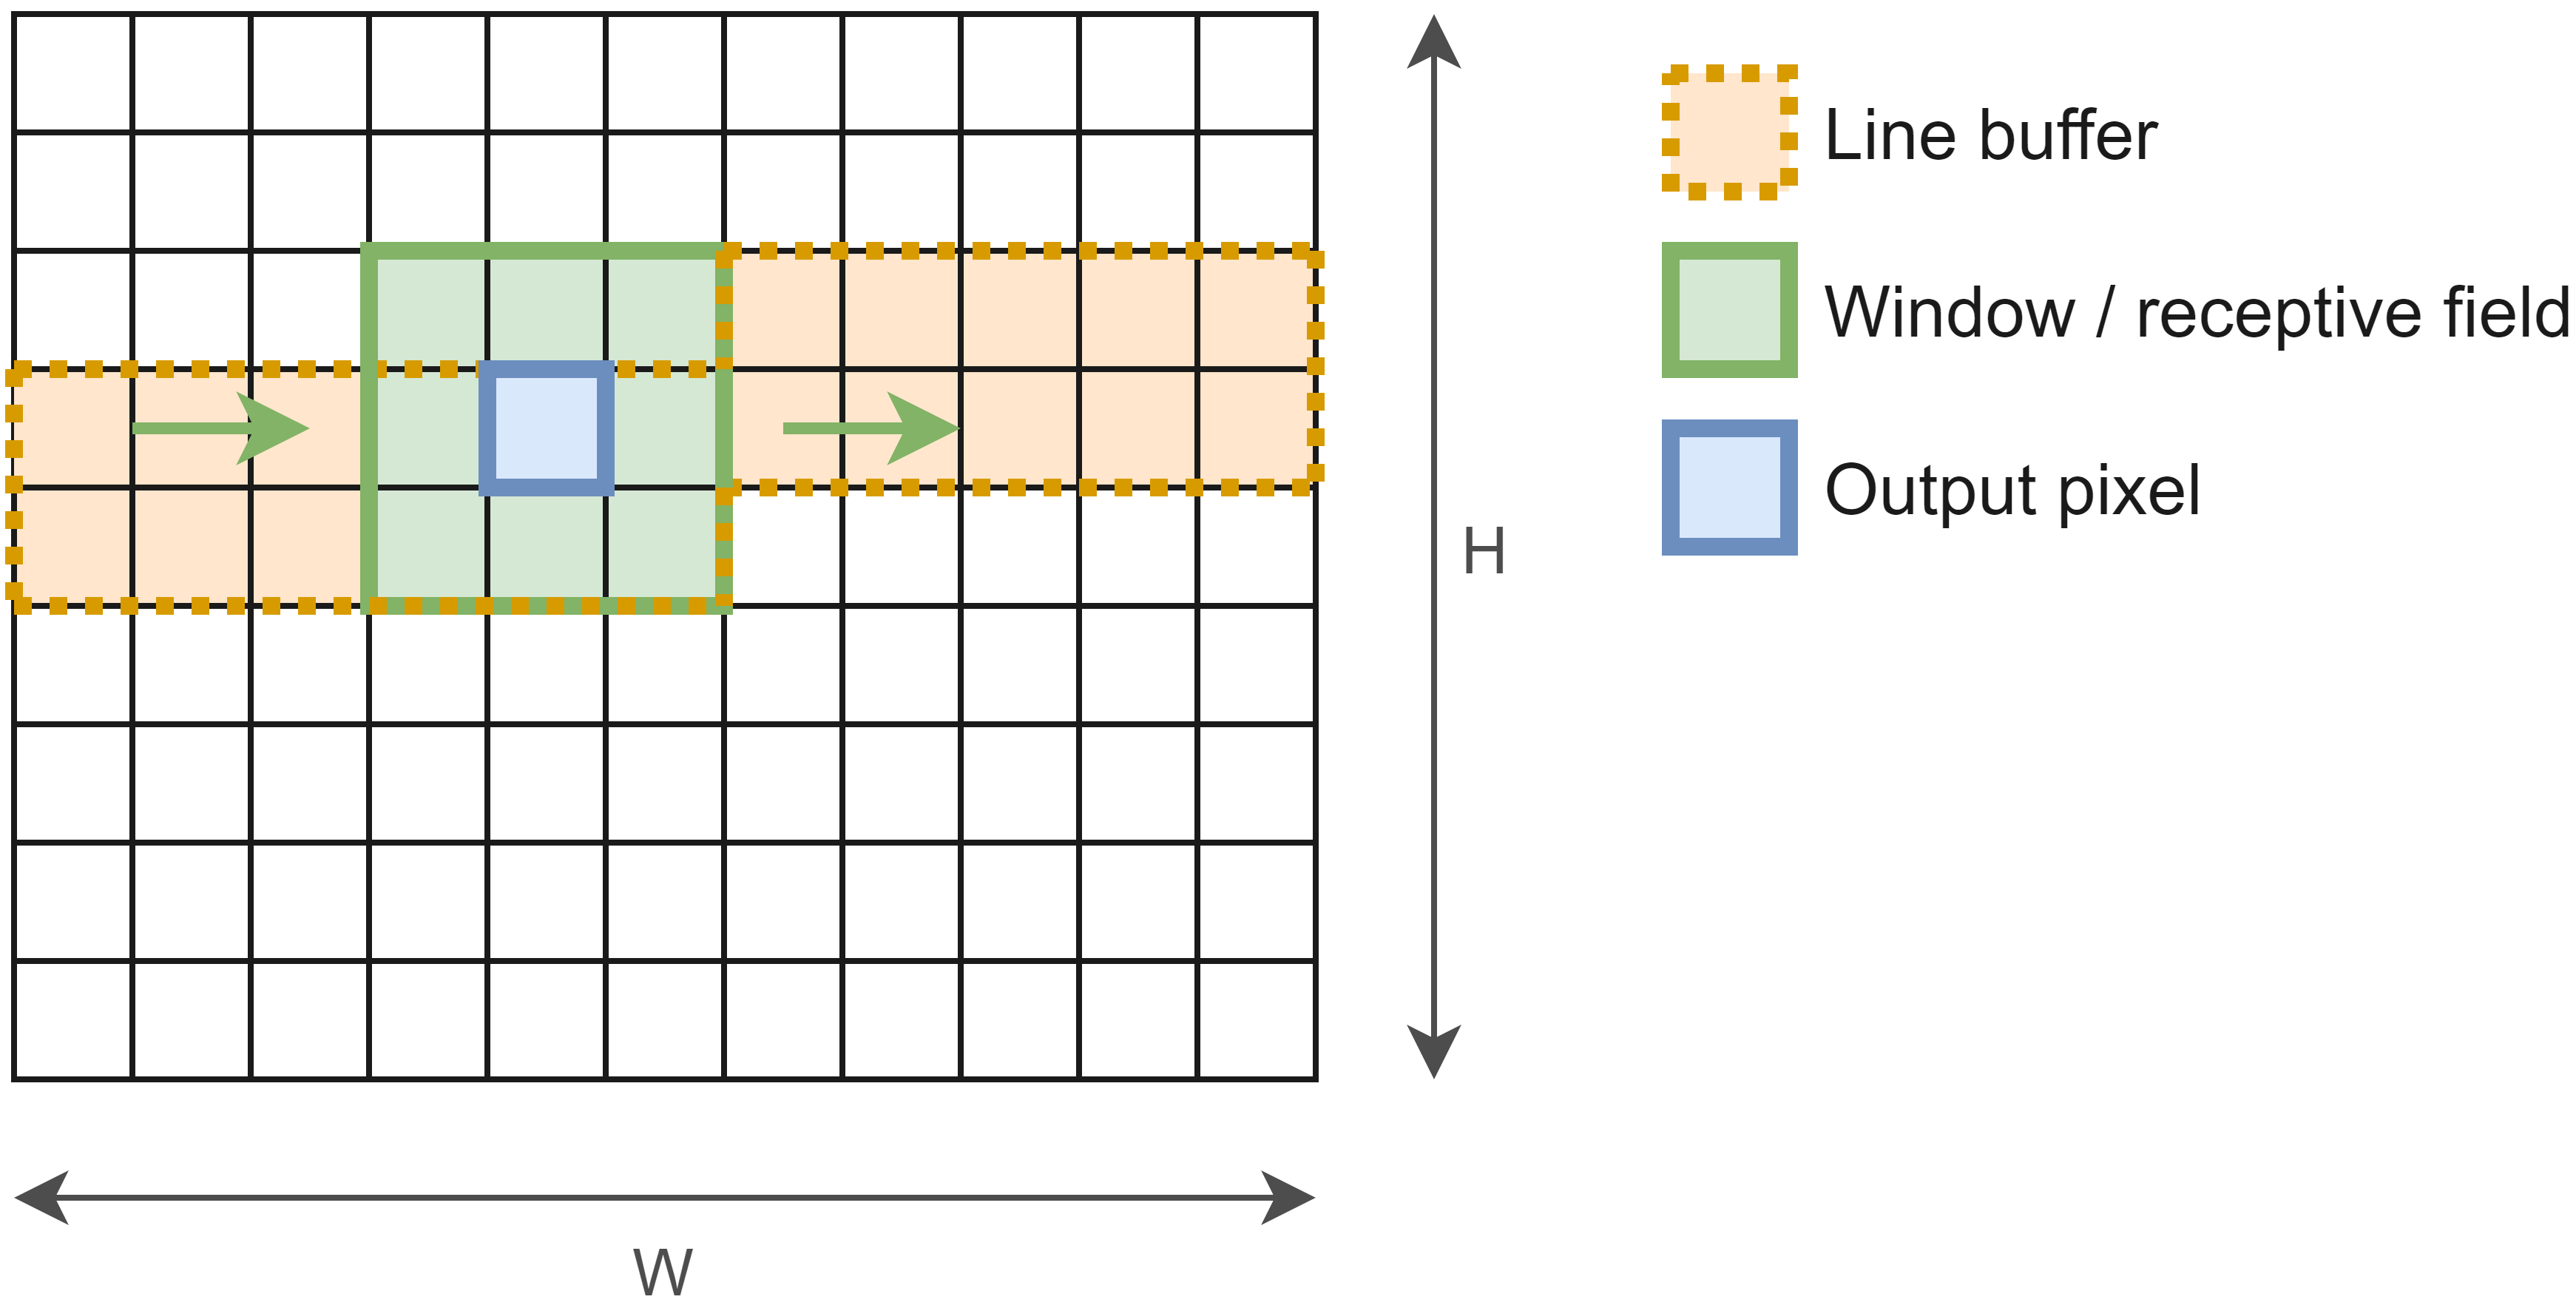
\includegraphics[width=0.8\textwidth]{hoorick2019-convolutions.png}
				\cite{hoorick2019convolution}
			\end{figuur}

			Another advantage of using these line buffers is that we can run the next operation upon the image once the previous operation is done with the lines.
			This is called pipelining, and it enables us to do multiple operations on an image at once with just a small interval between the operations.
			I have used pipelining in the VPU core wherever possible, because it is my goal to reduce image processing latency as much as possible.
			It is my goal to prove that FPGAs are viable for this purpose, so I want to illustrate it with good benchmarks.
			I managed to pipeline all the AXI stream operations, the image color operations, the Gaussian and Sobel filters and the thresholding.
			
			\bigskip

			Unfortunately, I could not apply pipelining to the Hough Transform because this operation needs to have computed all the votes in the accumulator of an image before it can proceed with thinning and sorting of the votes.
			This means that the Hough Transform takes up a lot of memory.
			In fact, I could not even fit the full voting accumulator for the Hough Transform on the FPGA because it used too much BRAM.
			For an image frame of 1280 by 720 pixels, the full accumulator would take up around \qty{6}{\mebi\bit} according to the formula in \verwijzingb{figuur}{Equation for the Hough accumulator size}.
			I needed to lower the theta resolution by two to make the accumulator small enough to fit in the memory.
			The standard full Hough Transform checks 180 angles, but with the reduced $\theta$ resolution it means that we will only check every other angle.
			Consequently, the needed space for the accumulator is halved and fits well within the total of \qty{4,9}{\mebi\bit} available the PYNQ-Z2, leaving room for other components.

			\begin{figuur}{Equation for the Hough accumulator size}

				\vspace{1ex}

				\begin{equation*}
					A_s = \lceil log_e(w) / log_e(2) \rceil \cdot \frac{\theta_{max} - \theta_{min}}{\theta_{res}} \cdot \sqrt{w^2 + h^2}
				\end{equation*}

				\vspace{2ex}

				\textit{Where $w$ and $h$ are the width and height of the input image}

			\end{figuur}

			We can see how much FPGA resources every image processing operation uses by viewing the post-implementation report in Vivado.
			The \textit{utilization} section reports the used resources for every component of the pipeline.

			\begin{tabel}{Resource Utilization per Image Operation}{l @{\extracolsep{\fill}} r r r r}
				\textit{Operation} & BRAM  ($\times$ \qty{18}{\kibi\bit})	& DRAM ($\times$ \qty{64}{\bit})	& DSP	& Generic LUTs	\tabularnewline
				\midrule
				BGR to HSV	& 	& 	& 6	& 391		\tabularnewline
				HSV Threshold	& 6	& 16	& 	& 87		\tabularnewline
				Gaussian Blur	& 5	& 32	& 39	& 3483	 	\tabularnewline
				Sobel Filter	& 3	& 	& 	& 410		\tabularnewline
				Sobel Threshold	& 	& 	& 	& 75		\tabularnewline
				Hough Transform	& 184	& 	& 7	& 27838		\tabularnewline
				Float to Fixed	& 	& 	& 3	& 457		\tabularnewline

			\end{tabel}

			I did not specifically include the shift registers in \verwijzingb{tabel}{Resource Utilization per Image Operation} because those can be implemented in non-SLICEM LUTs as well, of which there are plenty.
			We can confirm from this report that the Hough Transform is very memory intensive.
			The storage of the vote accumulator used a total of 92 RAMB36E1 blocks, resulting in a total of \qty{3312}{\kibi\bit} being instantiated for the Hough Transform alone.
			This is almost 70 percent of the total BRAM available on the FPGA.
			Convolution-based image operations like the Gaussian Blur and the Sobel Operator were implemented with very little memory required.
			This is because of the line buffers and aggressive pipelining.
			They hand over data to the next function after processing only a few lines, and thus not requiring much storage.

		\end{paragraaf}

		\clearpage

		\begin{paragraaf}{Communication Workflow between the PS and the PL}
			
			What makes the Zynq SoC appealing is that is has a hard-IP memory controller that is directly connected to the SDRAM.
			Therefore, the developer does not need to implement the DDR3 memory interface themselves.
			I used this benefit to my advantage; my strategy is to place the images into memory using the CPU and then access them using VDMA in the digital logic.
			This leaves the BRAM/DRAM available for the image processing logic.
			The VDMA IP Cores with the driving logic for the memory interface are supplied by Xilinx, requiring little work on my part to fetch the images in PL.

			\vspace{-0.6ex}
			\begin{figuur}{Classic hardware co-processing compared to FPGA co-processing}
				\singlespacing
				\includegraphics{coprocessing}
				\onehalfspacing
				\vspace{-2.3ex}
			\end{figuur}
			\vspace{-0.2ex}

			The way the memory is used on the Zynq-7000 with VDMA reminds me of using the OpenGL and Vulkan graphics APIs.
			With OpenGL, you would allocate 'textures' and other data the GPU needs in the host memory and then pass a reference to the data to the shader program that would run on the GPU.
			With Vulkan, this process would be a bit more detailed and you would have to manually specify how you would stream the textures/data to the VRAM before being able to access this data from the shader.
			And now, with Zynq, we would allocate the data in host memory, stream the data to the BRAM/DRAM using the VDMA and then run the kernel by setting the register.
			After the data is processed, the VDMA feeds the results back into the buffer in host memory that we allocated.
			I did a lot of graphics programming a few years back, so I was able to see the similarities between these practices and adapt them to FPGA co-processing.
			
			\bigskip

			The transaction between software and hardware starts by allocating memory in the host's SDRAM by using the Xilinx Runtime (XRT) framework.
			This space will be accessible by the Programmable Logic via the VDMA.
			First, we copy the image into this memory space in the driver software.
			Subsequently, we send the address pointer to the VDMA IP Core in the Programmable Logic over the general-purpose AXI-Lite bus so that it knows where the image is located.
			This VDMA component is connected to our VPU IP Core using an AXI Stream, and the VDMA will provide the image data over this stream as soon as it is available.
			Then, we send a command to the VPU IP Core over it's AXI-Lite interface that it can start processing the data.

			\vspace{-0.6ex}
			\begin{figuur}{Communication between Host and Accelerator in Co-processing Methodology}
				\singlespacing
				\begin{adjustbox}{width=\textwidth,center}
					\includegraphics{coproseq}
				\end{adjustbox}
				\onehalfspacing
				\vspace{-3.9ex}
			\end{figuur}
			\vspace{-0.2ex}

			Once the VPU IP Core is done with processing the data, it pulls the TLAST wire on the output AXIS interface high.
			This rising edge signals the VDMA that the data transfer is complete and that the receive channel should close.
			The output image data now resides at the output buffer location in the SDRAM and can be retrieved by the driver software running on the Processing System.
			A more detailed illustration of this process can be seen in \verwijzingb{figuur}{Communication between Host and Accelerator in Co-processing Methodology}.

		\end{paragraaf}

		\begin{paragraaf}{Status Indicator LEDs}

			The TUL Z2 development board has two user-controllable tri-color LEDs.
			I used these to display the status of the video processing driver.
			By default, the LEDs are set to shine red, like when the device is in standby mode.
			While processing a video frame, they are set to shine green.
			I used an AXI GPIO module in the programmable logic and connected it to board pins of the LEDS.
			This GPIO module can be accessed by the processor system and six bits (RGBRGB) can be written to it to update the light color.
			The names of the specific package pins that were used to drive these LEDs can be \verwijzingb{figuur}{Logical Schematic}.

		\end{paragraaf}

		\begin{paragraaf}{UART Peripheral}

			To give insight into the workings of the unit, it communicates its settings and results over a serial interface.
			The UART protocol was chosen for its simplicity and the availibility of existing solutions which can use it.

			\bigskip

			In the initial state, the TX line is pulled high by the peripheral.
			Once a data frame is to be sent, the TX line goes low, indicating a \textit{start bit}.
			After a time unit has passed, eight data bits are transmitted.
			Subsequently a parity bit is sent which is a logical 1 when the count of all bits that were 1 was even.
			Finally, the transmit line is pulled back into its initial high state, indicating a stop bit.
			The speed at which data is transferred, also referred to as the \textit{baud rate} is configured to be 230400 baud to allow for fast data transfer.
			At a processing speed of 40 video frames per second, approx. 3200 bits per second will be send over the serial connection, so we need the baud rate to be this high.
			The peripheral is configured to use 8 data bits, an even parity bit and one stop bit.

		\end{paragraaf}
	\end{hoofdstuk}

	\begin{hoofdstuk}{Programmable Logic Layer}

		\begin{paragraaf}{Video Processing Unit}

			% ----- Introductie; wat is HLS en Vitis Vision?
			I chose to implement the image processing stages using High Level Synthesis because Xilinx provides a well-designed OpenCV port that is tested and formally proven.
			This port was formerly called xfOpenCV prior to it being integrated into the Vitis standard libraries and being renamed to Vitis Vision.
			It is a clean-room implementation of OpenCV functions that includes instruction pragmas which tell the compiler how certain code should be synthesized to RTL.
			These pragmas include information on how certain loops should be unrolled and how variables can be synthesized to registers.
			The developer can write C++ code which specifies which AXI interfaces have to be created and which vision functions have to be applied.
			This code can be simulated on the developer's system using the official OpenCV library to verify the working of the code.
			Once verified, the code can be synthesized to a HDL and can be co-simulated to verify that the automatically generated HDL performs exactly like the original code.
			Finally, Vivado can synthesize the HDL to a netlist and implement it into an IP Core, which can be used in other projects.

			\vspace{1ex}
			\begin{figuur}{The IP core as seen in the block design}
				\centerline{
					%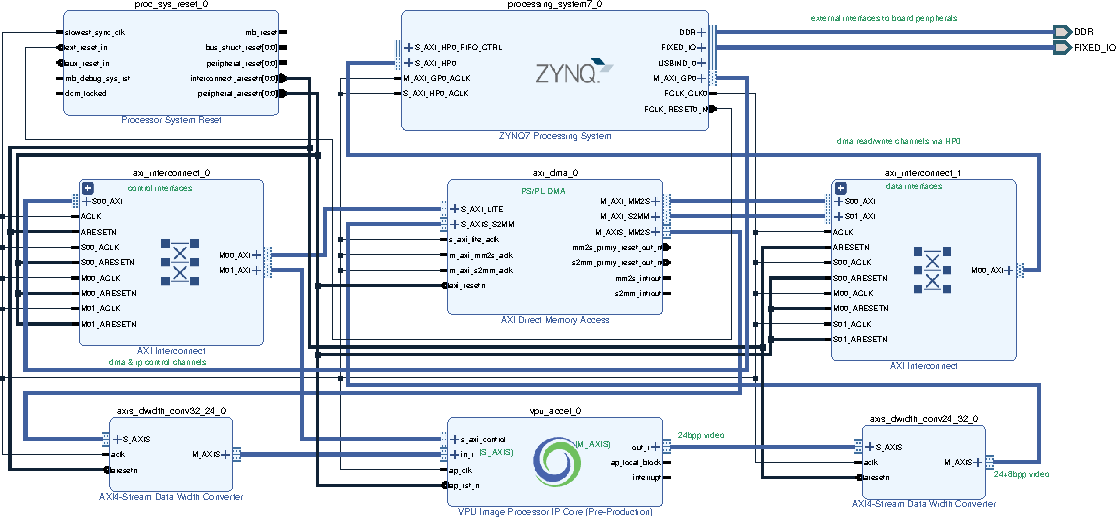
\includegraphics[width=0.76\textwidth, clip, trim=6.5cm 0.16cm 6.5cm 6.9cm]{hw-block-diagram-crop-asset.pdf}
					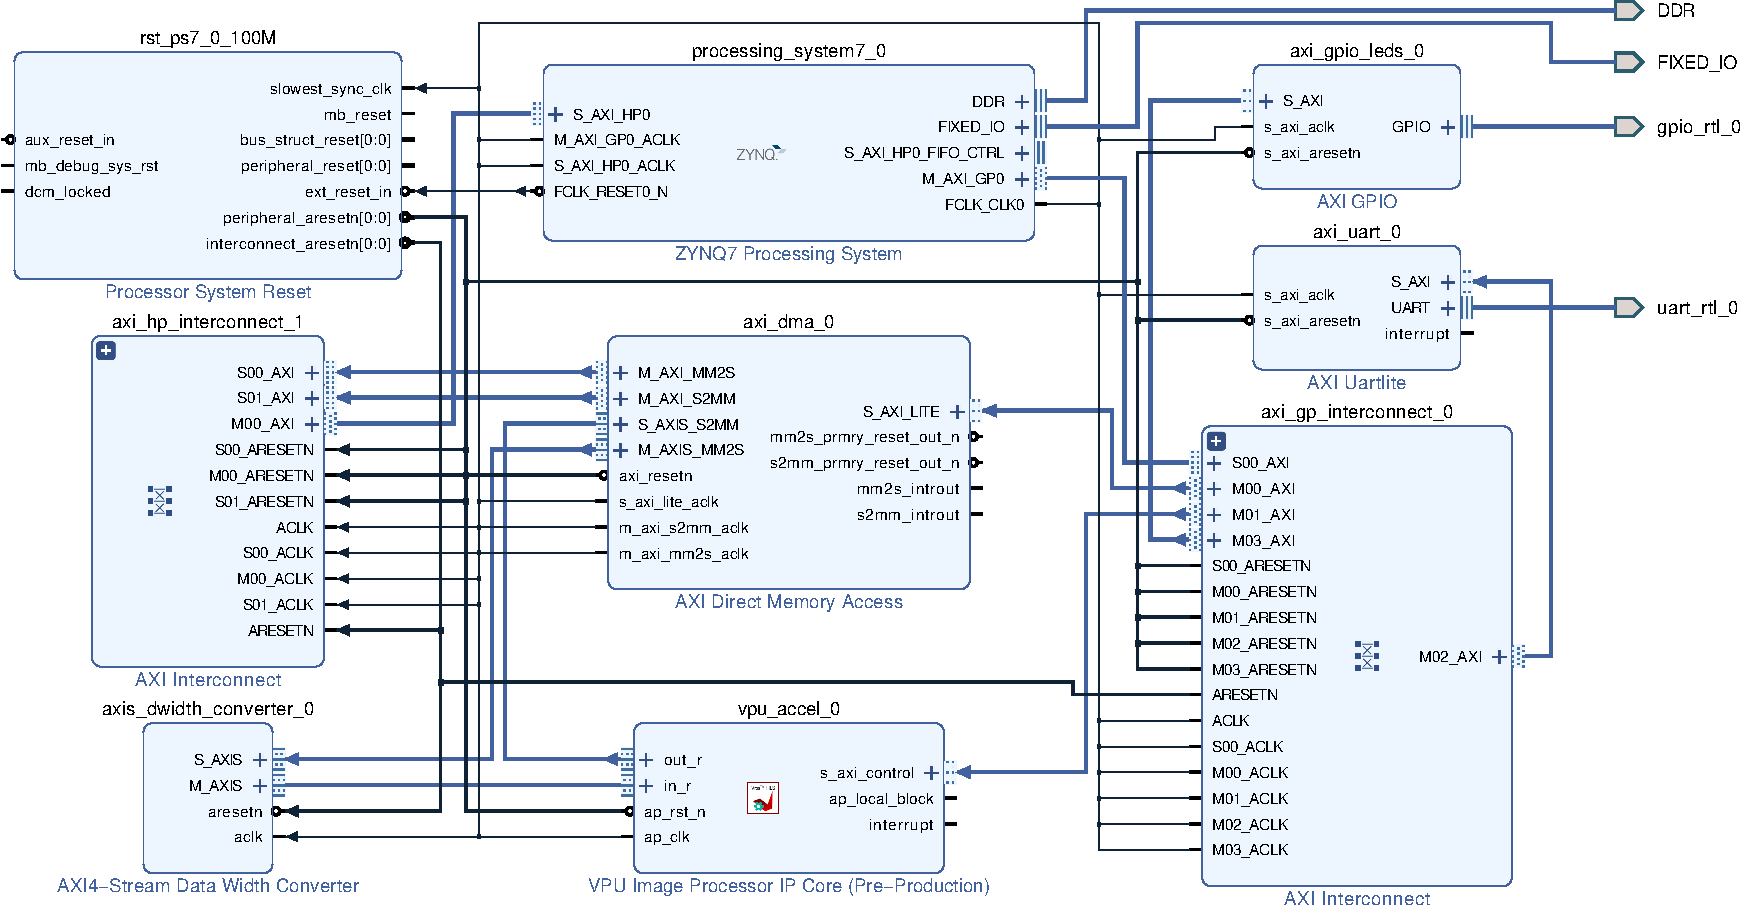
\includegraphics[width=0.76\textwidth, clip, trim=8.75cm 0.16cm 11.5cm 12.2cm]{hw-block-diagram-v2-crop-asset.pdf}
				}

				\vspace{3ex}

				{
				\small
				\begin{tabular}{l l l}
					\toprule
					Signal(s) & Width & Description \\
					\midrule
					in\_r & \qty{24}{\bit} & Image input stream (RGB-888 = 24bpp) \\
					out\_r & \qty{32}{\bit} & Detected lines output (Q10.22 pairs until TLAST) \\
					ap\_clk & - & Clock signal of 125 MHz \\
					ap\_rst\_n & - & Reset signal for reverting internal state \\
					s\_axi\_control & \qty{32}{\bit} data + \qty{6}{\bit} addr & Used to control and adjust detection parameters \\
					ap\_local\_block & - & Remains low as long as no deadlock occurs \\
					interrupt & - & Goes high when image has been processed \\
					\bottomrule
				\end{tabular}
				}
			\end{figuur}

			The video processing code that I wrote declares two AXI streams that are used to access the data and are implemented by Vitis as line-buffers.
			The first stream is configured as input and takes RGB888 pixels from the source image in row-major order.
			This data is fed into a sequence of Vitis Vision functions that make up the video processing pipeline as described in the research paper.
			The Houghlines function, which is the last function of this sequence, returns the detected lines in the image in floating point format.
			These lines are then converted to a \qty{32}{\bit} wide fixed point format and sent to the DMA.
			I chose to convert the values to fixed point because they are always in a predictable range.
			For example, the theta values which represent the line angles are always in radians between zero and $ \pi $ (not inclusive).
			This means that the integer part can only have a maximum value of three, while the decimal is very important and should be stored in higher resolution.
			For the $ \rho $ value of the line a similar concept is of use; the integer part of the value fits within the range of $ [-\delta, \delta) $ where $ \delta $ is the image diameter.
			I chose to use a Q10.22 fixed point value for outputting the line values from the video processing code because of multiple reasons.
			Firstly, it can hold a sign bit, which is important for the $ \rho $ value of the lines because it can be negative.
			Secondly, it has enough resolution for the integer part of the $ \rho $ values for images with our desired image resolution of 1280 by 720.
			And finally, it has enough resolution to accurately convey the decimal part of the $ \theta $ value of the lines.
			As described earlier, I halved the theta resolution of the Hough Transform, which reduces the number of possible values to well within the $ 2^{22} $ range.
			Alongside these two AXI streams, I declared an AXI-Lite interface with control registers.
			These control registers contain the parameters of the video processing functions, like the thresholds and a start/stop bit.
			The values can be adjusted by the software at runtime by writing new values to them.
			The main control register resides at offset 0x00 and can be used to start/stop the processing of the video by modifying the values seen in\verwijzingb{tabel}{Control register description}.
			The full list of registers available over the AXI-Lite bus is in\verwijzingb{tabel}{IP core register index}.

			\begin{table}[h]
				\centering
				\begin{tabularx}{0.9\textwidth}{p{8ex} c X c c c c} 
					Field &
					\makebox[2ex][l]{\rotatebox{60}{\small AUTO\_RESTART}} &
					&
					\makebox[2ex][l]{\rotatebox{60}{\small AP\_READY}} &
					\makebox[2ex][l]{\rotatebox{60}{\small AP\_IDLE}} &
					\makebox[2ex][l]{\rotatebox{60}{\small AP\_DONE}} &
					\makebox[2ex][l]{\rotatebox{60}{\small AP\_START}} \\
					\noalign{\vskip 0.8ex}\cline{2-7}
					Bit &
					\multicolumn{1}{|c|}{7} &
					6 \hfill ... \hfill 4 &
					\multicolumn{1}{|c}{3} &
					\multicolumn{1}{|c}{2} &
					\multicolumn{1}{|c}{1} &
					\multicolumn{1}{|c|}{0} \\
					\cline{2-7}\noalign{\vskip 0.8ex}  
					Access &
					\small R/W &
					\small &
					\small R &
					\small R &
					\small R &
					\small W \\\noalign{\vskip 0.8ex}
					Reset &
					\small 0 &
					&
					\small 1 &
					\small 1 &
					\small 0 &
					\small 0 \\
				\end{tabularx}
				\caption{Control register description}
				\label{tabel:Control register description}
			\end{table}

			\begin{tabel}{IP core register index}{l l r c l}
				Register & Offset & Width & Access & Description \\
				\midrule
				CTRL & 0x00 & 8 & R/W & Signals to control the operation \\
				IINH & 0x10 & 32 & W & Input image height in pixels (max. 720) \\
				IINW & 0x14 & 32 & W & Input image width in pixels (max. 1280) \\
				THRS & 0x20 & 8 & W & Threshold value for the HSV image segmentation \\
				GASZ & 0x21 & 8 & W & Sigma value of the Gaussian blur function \\
				THRE & 0x22 & 8 & W & Threshold value of the Sobel filter output \\
				THRH & 0x23 & 16 & W & Threshold value of the Hough votes \\

			\end{tabel}
			
			\bigskip

			Using the Vitis HLS application I synthesized the high level code to RTL and packaged it into an IP core.
			I incorporated this IP core into the block design using the Vivado IPI and connected it to the DMA component.
			The DMA component has a bus data width of \qty{32}{\bit} to match that of the Zynq PS/PL AXI HP port.
			Because the video processing logic image input stream is only \qty{24}{\bit} wide, I used an AXI data width converter to cut off the top bits.
			The software driver is configured to pad the output stream with zeroes up to this \qty{32}{\bit} width.
			From the software, we send the memory location of a RGB-888 video frame that is stored in the SDRAM to the DMA via its AXI-Lite port, which will initiate the transfer via the \qty{32}{\bit} wide bus to the converter, which, in turn, will ignore the padding by only transferring the first \qty{24}{\bit}.
			This step causes the data to become available on the input interface of the VPU core.
			Next, we set the \textit{AP\_START} and \textit{AUTO\_RESTART} bits of the memory-mapped control register of the VPU core via its AXI-Lite interface.
			This will toggle the VPU core into a mode where it automatically processes the data available on the input stream.
			The start/stop/etc control logic is implemented with the "return" pragma in the VPU code and is generated by Vitis, ensuring that it is correct.
			To express this in FPGA terminology, we can think of 'inference' of this control interface.
			Both the input and output stream interfaces have FIFO queues implemented as underlying buffers.
			I did this to deal with the backpressure of the data width converters; the VPU IP core can take multiple clock cycles to read/write to/from the streams, while the AXI infrastructure components always transfer one pixel per clock cycle.

		\end{paragraaf}

		\clearpage

		\begin{paragraaf}{Lane Detection Pipeline}

			In the research paper I went into detail about the different video processing techniques I wanted to use.
			I did have to reflect back on my choices because the proposed pipeline did
			\begin{wrapfigure}{r}{0.4\textwidth}
				\centering
				%\begin{center}
					\vspace{-1ex}
					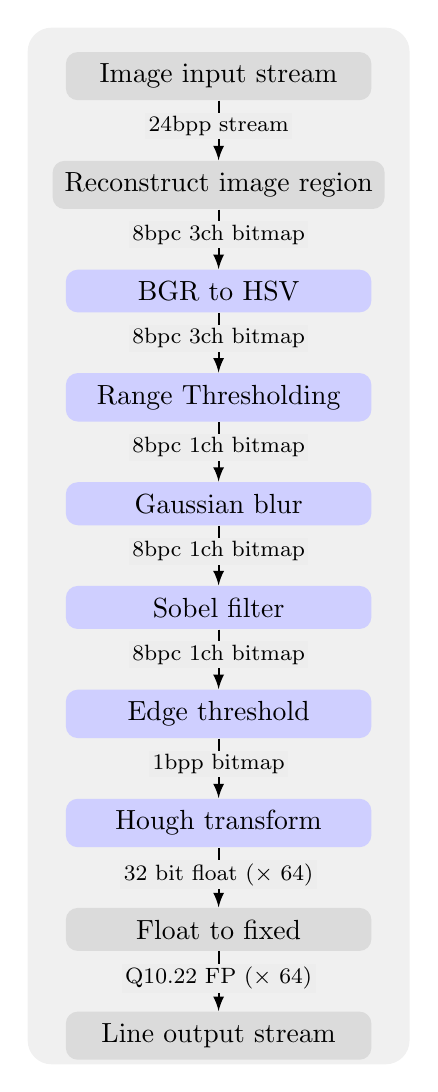
\begin{tikzpicture}

						% \tikzstyle exists, btw............

						\node (fig bg) [draw=none, fill=black!6, rounded corners=2ex, minimum width=0.4\textwidth, minimum height=87ex, inner sep=0, outer sep=0] at (0,0) {};
						\node (fig step 1) [draw=none, fill=black!14, rounded corners=1ex, minimum width=0.32\textwidth, inner sep=1ex, anchor=north, below=2ex of fig bg.north] {Image input stream};
						\node (fig step 2) [draw=none, fill=black!14, rounded corners=1ex, minimum width=0.32\textwidth, inner sep=1ex, anchor=north, below=5ex of fig step 1.south] {Reconstruct image region};
						\node (fig step 3) [draw=none, fill=blue!19, rounded corners=1ex, minimum width=0.32\textwidth, inner sep=1ex, anchor=north, below=5ex of fig step 2.south] {BGR to HSV};
						\node (fig step 4) [draw=none, fill=blue!19, rounded corners=1ex, minimum width=0.32\textwidth, inner sep=1ex, anchor=north, below=5ex of fig step 3.south] {Range Thresholding};
						\node (fig step 5) [draw=none, fill=blue!19, rounded corners=1ex, minimum width=0.32\textwidth, inner sep=1ex, anchor=north, below=5ex of fig step 4.south] {Gaussian blur};
						\node (fig step 6) [draw=none, fill=blue!19, rounded corners=1ex, minimum width=0.32\textwidth, inner sep=1ex, anchor=north, below=5ex of fig step 5.south] {Sobel filter};
						\node (fig step 7) [draw=none, fill=blue!19, rounded corners=1ex, minimum width=0.32\textwidth, inner sep=1ex, anchor=north, below=5ex of fig step 6.south] {Edge threshold};
						\node (fig step 8) [draw=none, fill=blue!19, rounded corners=1ex, minimum width=0.32\textwidth, inner sep=1ex, anchor=north, below=5ex of fig step 7.south] {Hough transform};
						\node (fig step 9) [draw=none, fill=black!14, rounded corners=1ex, minimum width=0.32\textwidth, inner sep=1ex, anchor=north, below=5ex of fig step 8.south] {Float to fixed};
						\node (fig step 10) [draw=none, fill=black!14, rounded corners=1ex, minimum width=0.32\textwidth, inner sep=1ex, anchor=north, below=5ex of fig step 9.south] {Line output stream};

						\draw [draw, -latex, thick] (fig step 1.south) -- (fig step 2.north) node[inner sep=0.3ex, pos=0.425, fill=black!7] {\footnotesize 24bpp stream};
						\draw [draw, -latex, thick] (fig step 2.south) -- (fig step 3.north) node[inner sep=0.3ex, pos=0.425, fill=black!7] {\footnotesize 8bpc 3ch bitmap};
						\draw [draw, -latex, thick] (fig step 3.south) -- (fig step 4.north) node[inner sep=0.3ex, pos=0.425, fill=black!7] {\footnotesize 8bpc 3ch bitmap};
						\draw [draw, -latex, thick] (fig step 4.south) -- (fig step 5.north) node[inner sep=0.3ex, pos=0.425, fill=black!7] {\footnotesize 8bpc 1ch bitmap};
						\draw [draw, -latex, thick] (fig step 5.south) -- (fig step 6.north) node[inner sep=0.3ex, pos=0.425, fill=black!7] {\footnotesize 8bpc 1ch bitmap};
						\draw [draw, -latex, thick] (fig step 6.south) -- (fig step 7.north) node[inner sep=0.3ex, pos=0.425, fill=black!7] {\footnotesize 8bpc 1ch bitmap};
						\draw [draw, -latex, thick] (fig step 7.south) -- (fig step 8.north) node[inner sep=0.3ex, pos=0.425, fill=black!7] {\footnotesize 1bpp bitmap};
						\draw [draw, -latex, thick] (fig step 8.south) -- (fig step 9.north) node[inner sep=0.3ex, pos=0.45, fill=black!7] {\footnotesize 32 bit float ($ \times $ 64)};
						\draw [draw, -latex, thick] (fig step 9.south) -- (fig step 10.north) node[inner sep=0.3ex, pos=0.45, fill=black!7] {\footnotesize Q10.22 FP ($ \times $ 64)};
					\end{tikzpicture}
				%\end{center}
				\vspace{-4ex}
				\caption{Detection Pipeline}
				\label{figuur:Detection Pipeline}
			\end{wrapfigure}
			not work as well as intended.
			Instead of $ k $-means image segmentation, I ended up segmenting the image using luminance thresholding, because this gave better results.
			White lane markings have low saturation and high luminance compared to the rest of the environment, which makes HSV segmentation an effective technique.
			The luminance thresholding is implemented by limiting the saturation and value parameters of an image in the HSV colorspace.
			To accomodate for this, I had to add a conversion step from the source colorspace, BGR, to HSV.
			The thresholding itself is done by the \textit{xf::cv::inRange} function, which sets all pixels outside of a certain threshold to black.

			\bigskip

			The complete sequence of image operations is visualized in \verwijzingb{figuur}{Detection Pipeline}.
			In this figure, the steps that I implemented myself are marked in black and the steps I used Vitis Vision functions for are marked in blue.
			The interim data types that were used for buffering data between operations are typed onto the arrows.
			An interesting thing to note is that the data types gradually get smaller up until the Hough transform; starting out with 24 bpp and ending on 1 bpp.
			This is indicative of what we are trying to accomplish: we are trying to minimize a full video frame to just edge pixels.
			
			\bigskip

			The final resulting data is a list of 32 lines that were detected in the image.
			Each line is expressed as a ($ \rho, \theta $) pair, which means that the logic will output 64 values per frame.
			The amount of lines that are output is fixed, because it is implemented in digital logic.
			Changing this amount requires resynthesizing digital logic.
			For now, 32 lines are more than enough.

			In software we will be able to smooth and stabilize these lines to find the average lane marking lines.

		\end{paragraaf}

	\end{hoofdstuk}

	\begin{hoofdstuk}{Processing System Layer}

		By default, a jumper is connected on the Z2 board that enables the Cortex-A9 to boot from the firmware on an SD card.
		I flashed a PetaLinux image with the PYNQ framework onto an SD card because this is the recommended software by the board manufacturer.
		The PYNQ framework (an abbreviation of "Python for Zynq") lets the developer use Python scripts to quickly prototype software that interacts with the programmable logic components.
		I used this framework to create a driver script that loads the design bitstream on to the FPGA and communicates with the components in digital logic.
		Another advantage of running the driver code on an embedded Linux system is that it comes with device drivers for external peripherals like webcams.
		This meant that I could attach a dashcam (a Logitech C270) and grab road images from it. For additional sample material, I wrote dashcam video to the SD card.

		\begin{paragraaf}{Driver}

			This Python script is responsible for setting up the components on the FPGA and offloading the video frames.
			It has a main loop that runs as long as the device is powered on and no error has occured.

			\begin{figuur}{Driver Activity Diagram}
				\singlespacing
				\centerline{
					\includegraphics{activity-diagram} 
				}
				\onehalfspacing
			\end{figuur}
			
			The main workflow of the driver script is illustrated in \verwijzingb{figuur}{Driver Activity Diagram}.
			The status update message and the result message are messages that are sent over the UART connection for debugging purposes.
			As can be seen, the light color of the LEDs is changed depending on whether a lane departure warning is emitted.

		\end{paragraaf}

		\begin{paragraaf}{Determining The Car Position}

			The last step of the video processing pipeline that is implemented in hardware is the Hough transform.
			This operation gives us up to 32 lines that were detected within the image.
			They are returned in ($ \rho , \theta $) format, where these two parameters represent a point on the sinusoidal plane.
			It is possible to quantize these coordinates to a line on the Cartesian plane in $y = \alpha x + \beta$ format, but I came up with a simple algorithm that does not require this.
			The algorithm can determine whether or not the car is about to leave the lane by taking into account the angles of both lines.

			\bigskip

			First, we categorize the 32 detected lines into two buckets; one for the left lane line and one for the right lane line.
			If the angle in radians of the detected line is higher than $\frac{\pi}{2}$ it is put into the left bucket, otherwise into the right bucket.

			\bigskip

			Then, we average the values from each bucket to one $\theta$ value.
			This is a precise lane line of the current video frame.
			To prevent inconsistencies and stabilize the readings over an extended period of time, a moving average is kept over the last five video frames.

			\bigskip

			Now that we have stable readings of the angles of the left and right lane lines, there's only one step left: detecting a lane departure.
			This is done by comparing the distance of each line to the center of the frame.
			If the distance between one of these lines and the center of the frame is double that of the other, we can say that a lane departure is about to happen.
			Tests on sample footage have confirmed that this technique is effective enough to meet requirements.

		\end{paragraaf}

		\begin{paragraaf}{Transmitting Results Over UART}

			For troubleshooting purposes, some internal values are transmitted over the UART connection.
			A technician can debug the device to view the algorithm settings and the results of a processed video frame.
			As mentioned in \verwijzingn{paragraaf}{UART Peripheral}, the UART connection is configured to send eight data bits per data frame.
			Because we need to send larger amounts of information than that, I have created an abstraction on top of this protocol which serializes \textit{packets} to data frames.
			These packets contain multiple fields with related information and are sent sequentially.
			Every type of packet has an identifier (\textit{opcode}) that is sent as an \qty{8}{\bit} integer before the data fields are sent.
			All data is little-endian.

			\begin{tabel}{Packet types}{l l l}
				Opcode & Name & Description \tabularnewline
				\midrule
				0x02 & Status Update & The device goes online/offline or a setting has changed \tabularnewline
				0x04 & Frame Processed & A frame has been processed, the detected lines are sent \tabularnewline
				0x08 & Departure Warning & The car is nearing the edge of the lane, a warning is sent \tabularnewline
			\end{tabel}

			In the packet descriptions below, the data fields of the packet are illustrated.
			The \textit{value} row indicates if the field has a fixed value.
			If a packet does not have a fixed length, the variable length is indicated by a field so that the total length can be calculated.

			The first packet is the Status Update packet.
			It is issued by the system whenever the video processing loop starts or stops, or whenever the algorithm settings change.
			The packet has a total length of 41 bits which are aligned in 6 bytes.
			The first value after the fixed opcode field is a boolean which indicates whether the video processing is currently active or not.
			Subsequent values are the settings that the lane detection pipeline is configured to use, including the certain thresholds that were used in stages of the algorithm.
			The Gaussian blur sigma value is the standard deviation of the Gaussian function that is used to generate the convolution kernel for the blur operation.
			It is a decimal value encoded in Q2.6 fixed point format and can range from zero to five.
			The rest of the values can be treated as signed integers.

			\begin{table}[htbp!]
				\centering
				\begin{tabularx}{0.9\textwidth}{p{8ex} X X X X X X} 
					Field &
					\makebox[2ex][l]{\rotatebox{60}{\small Hough Threshold}} &
					\makebox[2ex][l]{\rotatebox{60}{\small Edge Threshold}} &
					\makebox[2ex][l]{\rotatebox{60}{\small Gaussian Sigma}} &
					\makebox[2ex][l]{\rotatebox{60}{\small HSV Threshold}} &
					\makebox[2ex][l]{\rotatebox{60}{\small Is Processing?}} &
					\makebox[2ex][l]{\rotatebox{60}{\small Opcode}} \\
					\noalign{\vskip 0.8ex}\cline{2-7}
					Bit &
					\multicolumn{1}{|c}{40 \hfill ... \hfill 33} &
					\multicolumn{1}{|c}{32 \hfill ... \hfill 25} &
					\multicolumn{1}{|c}{24 \hfill ... \hfill 17} &
					\multicolumn{1}{|c}{16 \hfill ... \hfill 9} &
					\multicolumn{1}{|c}{8} &
					\multicolumn{1}{|c|}{7 \hfill ... \hfill 0} \\
					\cline{2-7}\noalign{\vskip 0.8ex}  
					Value &
					&
					&
					&
					&
					&
					\multicolumn{1}{c}{\small 0x02} \\
				\end{tabularx}
				\caption{Status update packet description}
				\label{tabel:Status update packet description}
			\end{table}
			
			Detection results are sent over UART in the Frame Processed packet.
			This packet has a variable length depending on how many lines were detected, indicated by the \textit{Size} field.
			The total packet length in bytes is twice the \textit{Size} plus two.
			After the \textit{Size} field, an array of 16 bit wide integers is transmitted.
			The lower eight bits of this integer represent the $\rho$ value of the line in Q7.1 format and the upper eight bits are the $\theta$ value of the line in Q2.6 format.
			The rationale behind the resolutions of the fixed point integers is explained in \verwijzingn{paragraaf}{Video Processing Unit}.

			\begin{table}[htbp!]
				\centering
				\begin{tabularx}{0.9\textwidth}{p{8ex} X X X} 
					Field &
					\makebox[2ex][l]{\rotatebox{60}{\small Line\textsubscript{n} }} &
					\makebox[2ex][l]{\rotatebox{60}{\small Size}} &
					\makebox[2ex][l]{\rotatebox{60}{\small Opcode}} \\
					\noalign{\vskip 0.8ex}\cline{2-4}
					Bit &
					\multicolumn{1}{|c}{$15 + 16_n$ \hfill ... \hfill 16} &
					\multicolumn{1}{|c}{15 \hfill ... \hfill 8} &
					\multicolumn{1}{|c|}{7 \hfill ... \hfill 0} \\
					\cline{2-4}\noalign{\vskip 0.8ex}  
					Value &
					&
					&
					\multicolumn{1}{c}{\small 0x04} \\
				\end{tabularx}
				\caption{Frame processed packet description}
				\label{tabel:Frame processed packet description}
			\end{table}

			When the car is about to depart the lane, a Departure Warning packet is sent.
			Except for the opcode, this packet only contains one bit that indicates whether a warning has been issues or not.
			Therefore, the packet has a fixed length of 9 bits that is aligned into 2 bytes.

		\end{paragraaf}

	\end{hoofdstuk}
	
	\begin{hoofdstuk}{Software Layer}

		This chapter describes the working of the Remote Control application.
		It is meant for troubleshooting the system from an external workstation like a laptop/desktop computer.
		After the system is connected to this workstation via its serial port, the mechanic can start this application to read information in real-time.
		On its main GUI window, the application displays the algorithm settings and the live detection results.
		\begin{figuur}{Class Diagram of the Remote Control Application}
			\singlespacing
			\centerline{
				\includegraphics{class-diagram}
			}
			\onehalfspacing
		\end{figuur}

		\begin{paragraaf}{User Interface}

			The user interface was coded in the C++ language using the \textit{gtkmm} library, because I think that an object oriented language lends itself better to GUI programming than an imperative language like C does.
			Widgets of the user interface are represented as objects and can share code through inheritance.
			An example of this is the \textit{PreviewArea} widget I created; it overrides \textit{Gtk::DrawingArea} but it overrides some functions to add new functionality for drawing our own data to the screen.
			I left out the dependencies on \textit{gtkmm} in the previous class diagram and specified them in \verwijzingb{figuur}{Dependencies on Gtkmm}.
			
			\vspace{-1.5ex}
			\begin{figuur}{Dependencies on Gtkmm}
				\singlespacing
				\centerline{
					\includegraphics{class-diagram-deps}
				}
				\onehalfspacing
			\end{figuur}

			Another reason why I used object oriented programming paradigms was to simplify the reading of the different packet types; abstraction comes in handy when representing the packet inheritances.
			As can be seen in \verwijzingb{figuur}{Class Diagram of the Remote Control Application}, the different packet types override the abstract \textit{UartPacket} base class.

			\bigskip

			The InformationWindow class has many fields like input fields and labels that I did not include in the class diagram to prevent cluttering it.
			These fields are created when the window is created, and they are filled with values when data is received via the \textit{on\_*\_update(\textellipsis)} methods.

			\clearpage

			When a status update packet is passed to the \textit{on\_state\_update(\textellipsis)} method, the fields under the \textit{Device status} section are updated to reflect the latest settings of the device.
			A frame processed packet has no effect on the window itself, but is passed on to the PreviewArea element.
			The preview area is a rectangle interface element with a gray background and a fixed aspect ratio based on the resolution of the video.
			
			\vspace{-0.5ex}
			\begin{figuur}{Information Window of the Remote Control Application}
				\singlespacing
				\centerline{
					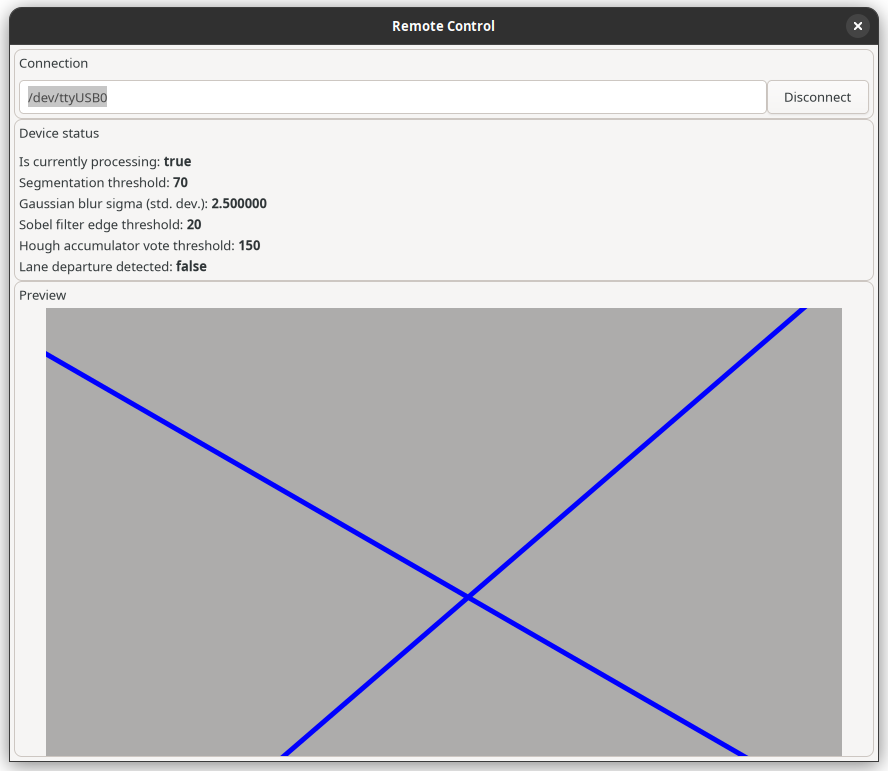
\includegraphics[width=0.9\textwidth]{rc-gui.png}
				}
				\onehalfspacing
			\end{figuur}

			Upon receiving a \textit{FrameProcessedPacket}, the preview area quantizes the sinusoidal lines from the packet back to lines in the Cartesian space.
			For each of these Cartesian lines, the intersections of the line with the rectangle element borders get calculated.
			Finally, lines are drawn on the screen between these intersections.
			If a departure is detected, the lines are drawn in red.
			Otherwise, they are drawn in blue.
			In \verwijzingb{figuur}{Information Window of the Remote Control Application} a normal situation is depicted wherein the car is driving within a lane.

		\end{paragraaf}

		\begin{paragraaf}{Serial Interface}

			The UART output from the system can be connected to a serial port of the workstation.
			In userspace, this serial port is usually available as a virtual device.
			On POSIX compliant operating systems it is available as \textrm{/dev/tty\textsubscript{N}} and on Windows NT and later as \textrm{COM\textsubscript{N}}.
			I added a text input field to the information window where the path to the virtual device can be specifed.
			Once the address has been entered, the \textit{Connect} button next to the input field can be clicked to instantiate the connection.
			A background thread is created to prevent the GUI from freezing while I/O operations are being executed.
			In this background thread, the virtual serial device is opened and the thread enters a loop that keeps reading incoming data until the connection is closed.
			The opening of the serial connection is done using the Unix \textit{termios} API.
			I used \textit{termios} because it allows easy configuration of the data bit amount and the parity bit setting.
			The reading of the serial device is done using the standard Unix system call \textit{read} in blocking fashion to give the thread a chance to idle when no data is available.
			This blocking call is indicated in \verwijzingb{figuur}{Serial Connection Activity Diagram} in red color.
			\verwijzingb{figuur}{Serial Drivers in Unix-based Systems} gives an overview of the layers behind the drivers.
			In the remote control application, I configure the TTY layer settings and use the user space layer for reading/writing.
			I do not use the line discipline layer because the bytes need to be transferred raw, no control codes or characters need to be parsed.

			\bigskip
			\begin{figuur}{Serial Drivers in Unix-based Systems}
				\vspace{-5ex}
				\singlespacing
				\centerline{
					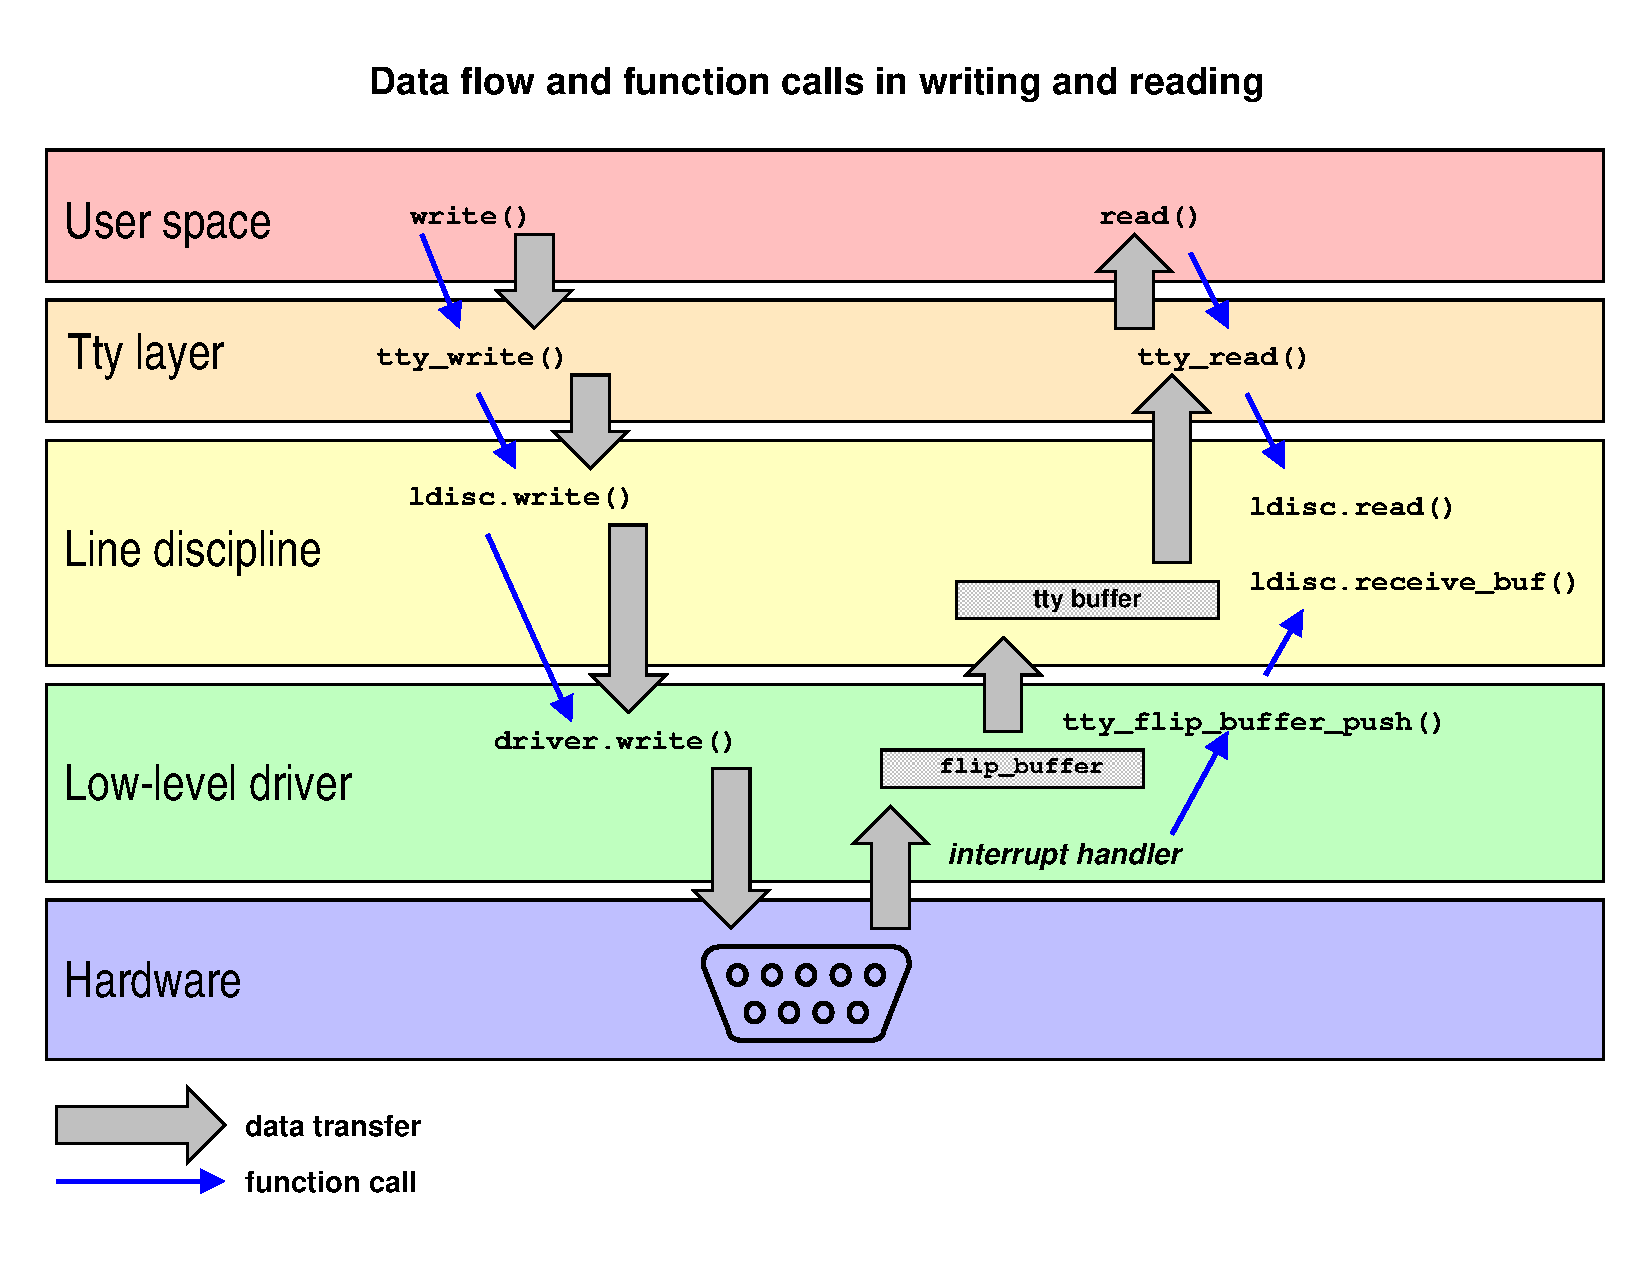
\includegraphics[width=0.8\textwidth, clip, trim=0cm 1cm 0cm 0.1cm]{rubini2006-img1.pdf}
				}\vspace{-1.2ex}\cite{rubini2006serial}\vspace{-0.7ex}
				\onehalfspacing
			\end{figuur}
			
			After the data has been read into a buffer, a derived \textit{UartPacket} object is created depending on the opcode of the packet.
			The fields of this object are set to the received values.
			Then, the packet gets added to a single-ended FIFO queue that is shared with the GUI thread.
			A mutex makes sure that this queue is only accessed by one thread at a time.
			After parsing all received data from the buffer into packet objects and adding them to the queue, the serial thread dispatches a signal to the GUI thread that new data is available.
			The data received callback in the GUI thread reads and removes all data packets from the queue and passes them to the information window, where they are handled as previously described.

			\clearpage

			\begin{figuur}{Serial Connection Activity Diagram}
				\vspace{-5ex}
				\singlespacing
				\centerline{
					\includegraphics{activity-diagram-serial}
				}
				\onehalfspacing
			\end{figuur}
		\end{paragraaf}

	\end{hoofdstuk}

	\begin{hoofdstuk}{Benchmarks}

		The reason of doing the heavy processing in hardware is to gain a speed advantage over software implementations.
		I have set up benchmarks in which I have compared the performance of the test program that I created as part of the research phase to OpenCV and finally to the FPGA implementation.
		Besides processing speed, I will also compare the power draw and efficiency of the different solutions.

		\begin{paragraaf}{Power Efficiency}

			Using hardware cosimulation in Vitis, it is possible to estimate the power draw of the FPGA chip.
			However, these metrics only take into account the FPGA fabric and not the ARM Cortex processor that is also embedded in the Zynq package.
			In Vivado, the power estimation report tool \textit{does} try to take into account the power draw of the processing system.
			This is marked in~\verwijzingb{figuur}{Total SoC Power Estimation}~with the PS7 label.
			However, since it does not know the code that will run on the processor and thus cannot estimate the processor load, it presumes a constant load of 50 percent.
			This is confirmed to be the case in~\verwijzingb{figuur}{CPU Power Estimation}.
			I think it gives more insight to compare only the metrics of the actual video processing logic between solutions because the driver code is unpredictable.
			Therefore, I will only compare the power consumption of the accelerator chips (GPU, FPGA) with each other.

			\vspace{1.5ex}
			\begin{figuur}{Total SoC Power Estimation}
				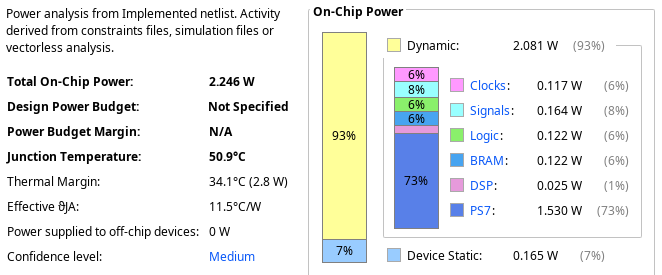
\includegraphics[width=0.85\textwidth]{vivado-power.png}
			\end{figuur}
			\begin{figuur}{CPU Power Estimation}
				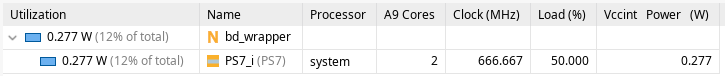
\includegraphics[width=\textwidth]{vivado-power-ps.png}
			\end{figuur}

			To benchmark the power consumption OpenCV reference code from my HLS testbenches, I used the AMD ROCm SMI tools.
			This library could read the power draw as reported by my iGPU.
			Note that my iGPU was not dedicated to the CV code alone; it was also used by other programs like my desktop environment.
			For this reason, the power draw is an estimation and should not be interpreted as being accurate.

		\end{paragraaf}

		\begin{paragraaf}{Execution Speed}

			It is possible to calculate the precise execution speed of the video processing logic by looking at the number of clock cycles needed for the pipelines to finish.
			The time in seconds can be calculated by dividing the number of clock cycles with the system clock speed of \qty{125}{\mega\hertz}.
			However, we have to take into account that, due to pipelining, the top left pixel of an image is transmitted (but also received) earlier than the bottom right pixel.
			The \textit{minimum latency} is the time between the transmission and return of the first pixel.
			The \textit{maximum latency} is the time spent between the transmission of the first pixel and the receiving of the last pixel.
			Thus, the maximum latency is a good metric to use for measuring the processing time of a single frame.
			For the whole video processing pipeline, including writing/reading image data to/from the local memory, the required cycles per operation is 1119344, which translates to \qty{11.19}{\milli\second}.

			\begin{figuur}{Vitis Timing Report for the VPU Logic}
				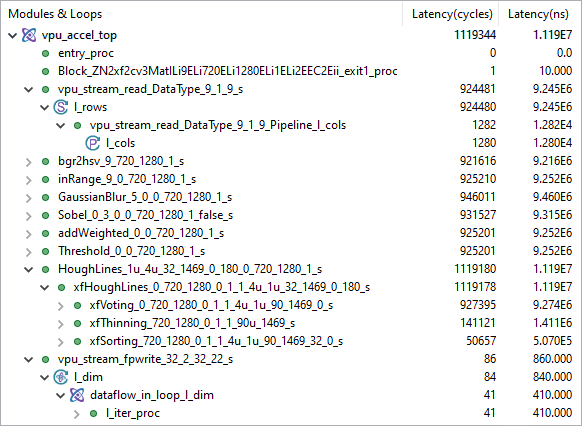
\includegraphics[width=0.7075\textwidth]{vitis-timing-bad-quality.png}
			\end{figuur}

			However, we also have to take into account the run time of the driver logic.
			I wrote the simple driver code using the PYNQ framework as it came preinstalled on the development board.
			The PYNQ framework is meant for rapid prototyping and is not meant for high performance situations.
			Instead of writing a barebones low-level application to run directly on the ARM Cortex core, PYNQ offers a Linux-based OS with a Python interpreter that can access the XRT and can interface with the FPGA hardware.
			When measuring the run time of the Python driver code, it took \qty{26.6}{\milli\second} ± \qty{443}{\micro\second} (mean std. dev. over 500 iterations) for the complete handling and processing of an image.
			As this is more than twice the total latency of the image processing alone, I suspect that the framework handles the memory operations inefficiently.
			Nevertheless, the frames per second that the code is able to process is still higher than that of a studio movie, so I'm quite happy with the speed of execution.

			\bigskip

			To measure the reference OpenCV execution speed, I used the \textit{TickMeter} class because it is part of the OpenCV core.
			I figured it would be better to use standardized methods than to roll my own.
			By using the TAPI introduced in OpenCV 3, I only had to make one change to my existing host code to run it on my iGPU: change the \textit{Mat} data type to \textit{UMat}.
			This data type is a generic one that can hold the data in the VRAM behind abstraction.
			I ran the reference programs on my laptop with a Ryzen 5 2500U with integrated graphics.

			\bigskip
			\vspace{-0.5ex}

			For running the OpenCV reference program, I isolated four CPU cores from the OS scheduler and dedicated them to the program.
			I also measured the performance of the test implementation (aka "Lane Program", I didn't have much inspiration for its name) that I made during the research phase of the project.
			This program is executed on the CPU and is only capable of using a single thread.
			For running the Lane Program, I dedicated one of the isolated cores to it.
			Except for the raw FPGA implementation, for which we can calculate the latency exactly, I ran all tests 500 times and calculated the average run time and standard deviation between run times.

			\bigskip
			\vspace{-1.5ex}

			\begin{tabel}{Performance comparison per platform}{l @{\extracolsep{\fill}} S[table-format=3.1]S[table-format=3.1]}
				Platform & {Average (ms)} & {Standard Deviation (ms)} \tabularnewline
				\midrule

				FPGA (raw)		& 11.2		& {-} 		\tabularnewline
				FPGA (co-processing)	& 26.6		& 0.443		\tabularnewline
				Reference OpenCV (CPU)	& 72.2		& 1.801		\tabularnewline
				Reference OpenCV (GPU)	& 14.2		& 0.794		\tabularnewline
				Reference Lane Program	& 382.7		& 13.81		\tabularnewline

			\end{tabel}

			\begin{figuur}{Bar chart visualization of Table \getrefnumber{tabel:Performance comparison per platform}}
				\centerline{
					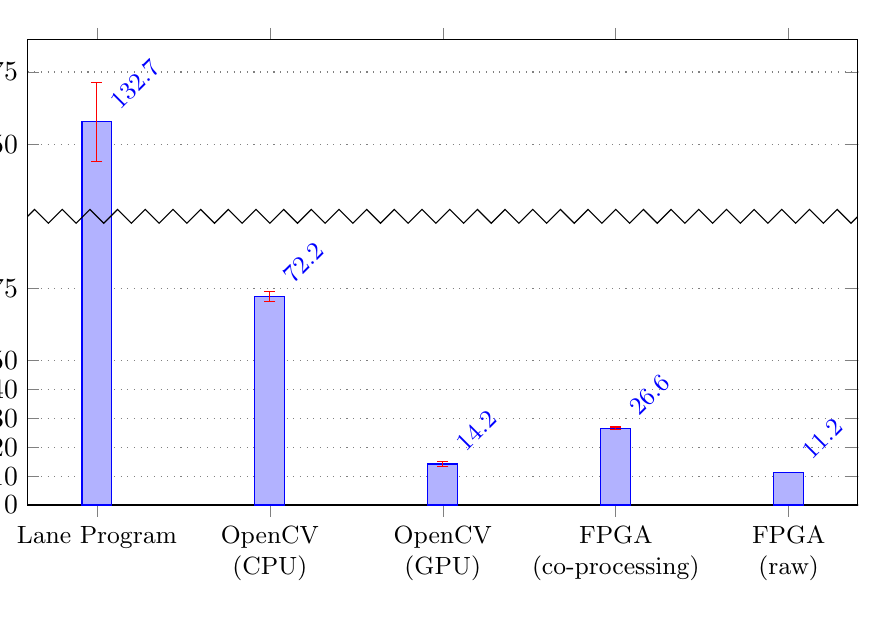
\begin{tikzpicture}[trim axis left, trim axis right]
					\begin{axis}[
						width=\textwidth,
						height=49.5ex,
						ybar,
						ymin=0,
						bar width=2.5ex,
						ylabel={
							milliseconds per execution \\
							\textit{(less is better)}
						},
						ylabel style={
							align=center,
							yshift=1ex
						},
						/tikz/every pin/.style={align=center},
						symbolic x coords={
							Lane Program,
							OpenCV (CPU),
							OpenCV (GPU),
							FPGA (coprocessing),
							FPGA (raw)
						},
						xtick=data,
						ytick=      {0, 10, 20, 30, 40, 50, 75, 125, 150},
						yticklabels={0, 10, 20, 30, 40, 50, 75, 350, 375, 400},
						x tick label style={align=center, font=\small},
						xticklabels={
							FPGA\\(raw),
							FPGA\\(co-processing),
							OpenCV\\(GPU),
							OpenCV\\(CPU),
							Lane Program
						},
						grid style={dotted, gray},
						ymajorgrids=true,
						nodes near coords,
						every node near coord/.append style={
							font=\small,
							align=left,
							rotate=45,
							anchor=south west,
							xshift=1.25ex,
							yshift=-1.5ex
						}
					]
						\addplot+[
							%restrict y to domain=0:100,
							error bars/error bar style={red},
							error bars/.cd, y dir=both, y explicit
						] coordinates {
							(FPGA (raw),		11.2)
							(FPGA (coprocessing),	26.6) +- (0, 0.443)
							(OpenCV (GPU),		14.2) +- (0, 0.794)
							(OpenCV (CPU),		72.2) +- (0, 1.801)
							(Lane Program,		132.7) +- (0, 13.81)
						};
					\coordinate (V) at (axis cs:Lane Program,100);
					\coordinate (H1) at (rel axis cs:0,0);
					\coordinate (H2) at (rel axis cs:1,0);
					\draw[black] decorate [decoration={zigzag}] {(V -| H1) -- (V -| H2)};
					\end{axis}
				\end{tikzpicture}
				}
				\vspace{-1ex}
			\end{figuur}

		\end{paragraaf}

	\end{hoofdstuk}
	
	% Bibliography page
	\begin{hoofdstuk}{References}

		\printbibliography[heading=none]

	\end{hoofdstuk}

	\begin{appendices}
		\begin{hoofdstuk}{Enlarged Figures}
			\begin{paragraaf}{Integrated Block Design Diagram}
				\vspace{1cm}

				%\centerline{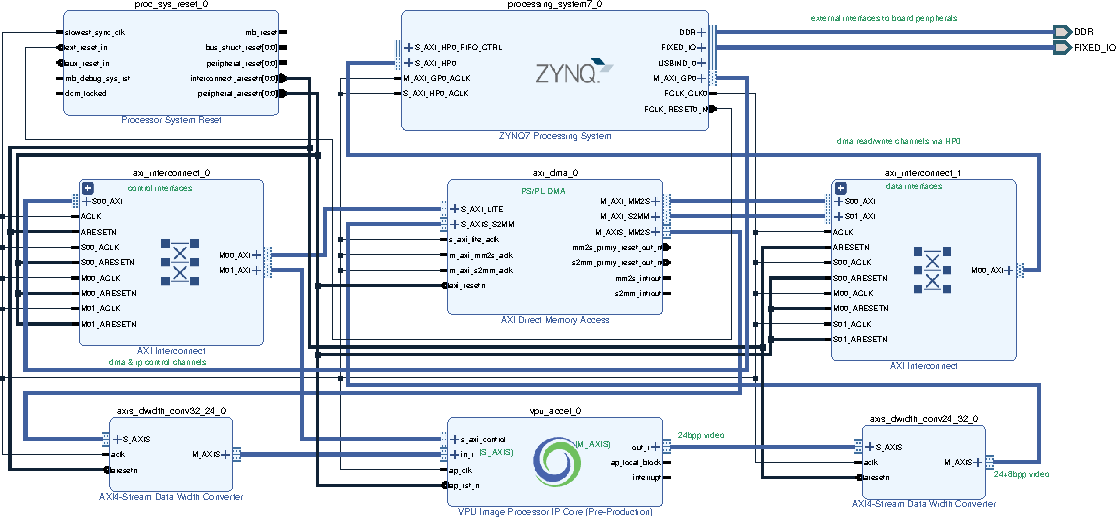
\includegraphics[angle=90, origin=c, clip, trim=9.45cm 0 0 0, width=1.25\textwidth]{hw-block-diagram-crop-asset.pdf}}
				%\clearpage
				%\centerline{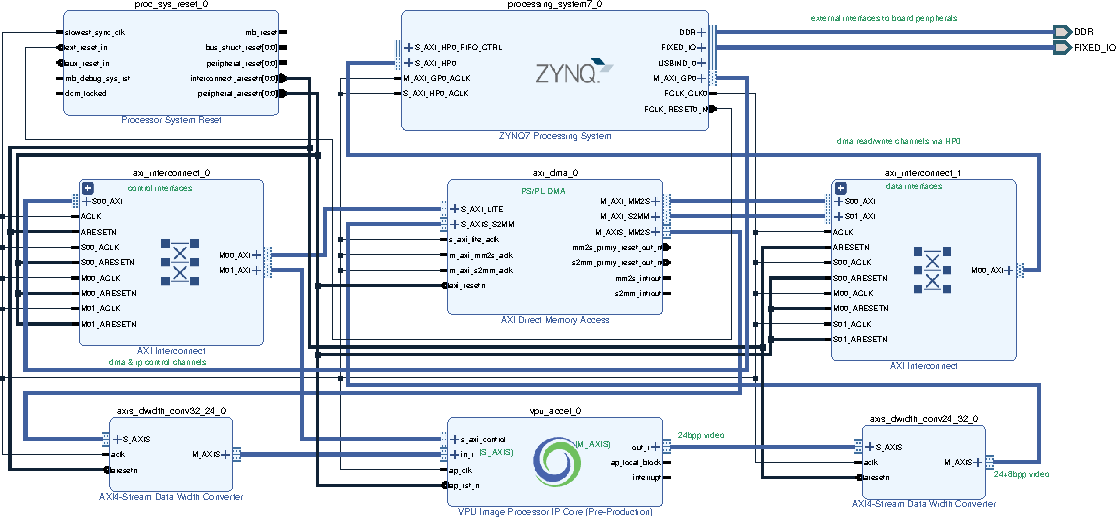
\includegraphics[angle=90, origin=c, clip, trim=0 0 9.45cm 0, width=1.25\textwidth]{hw-block-diagram-crop-asset.pdf}}
			
				% --- 14.75 * 2 = 29.5

				\centerline{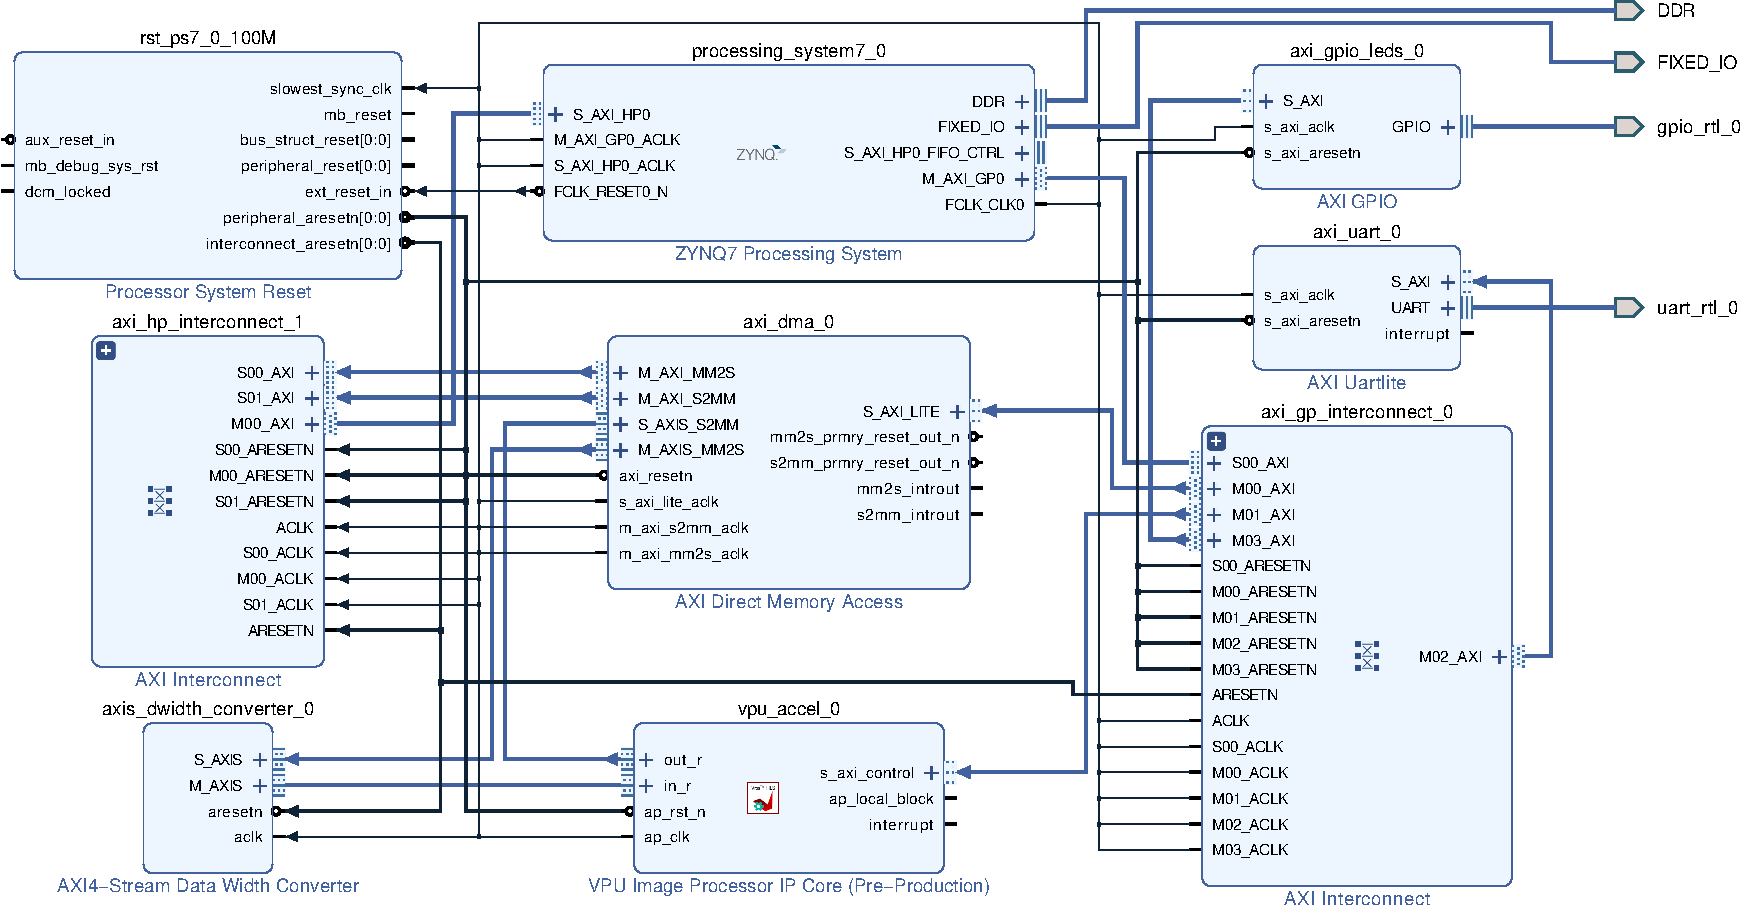
\includegraphics[angle=90, origin=c, clip, trim=12.90cm 0 0 0, width=1.25\textwidth]{hw-block-diagram-v2-crop-asset.pdf}}
				\clearpage
				\centerline{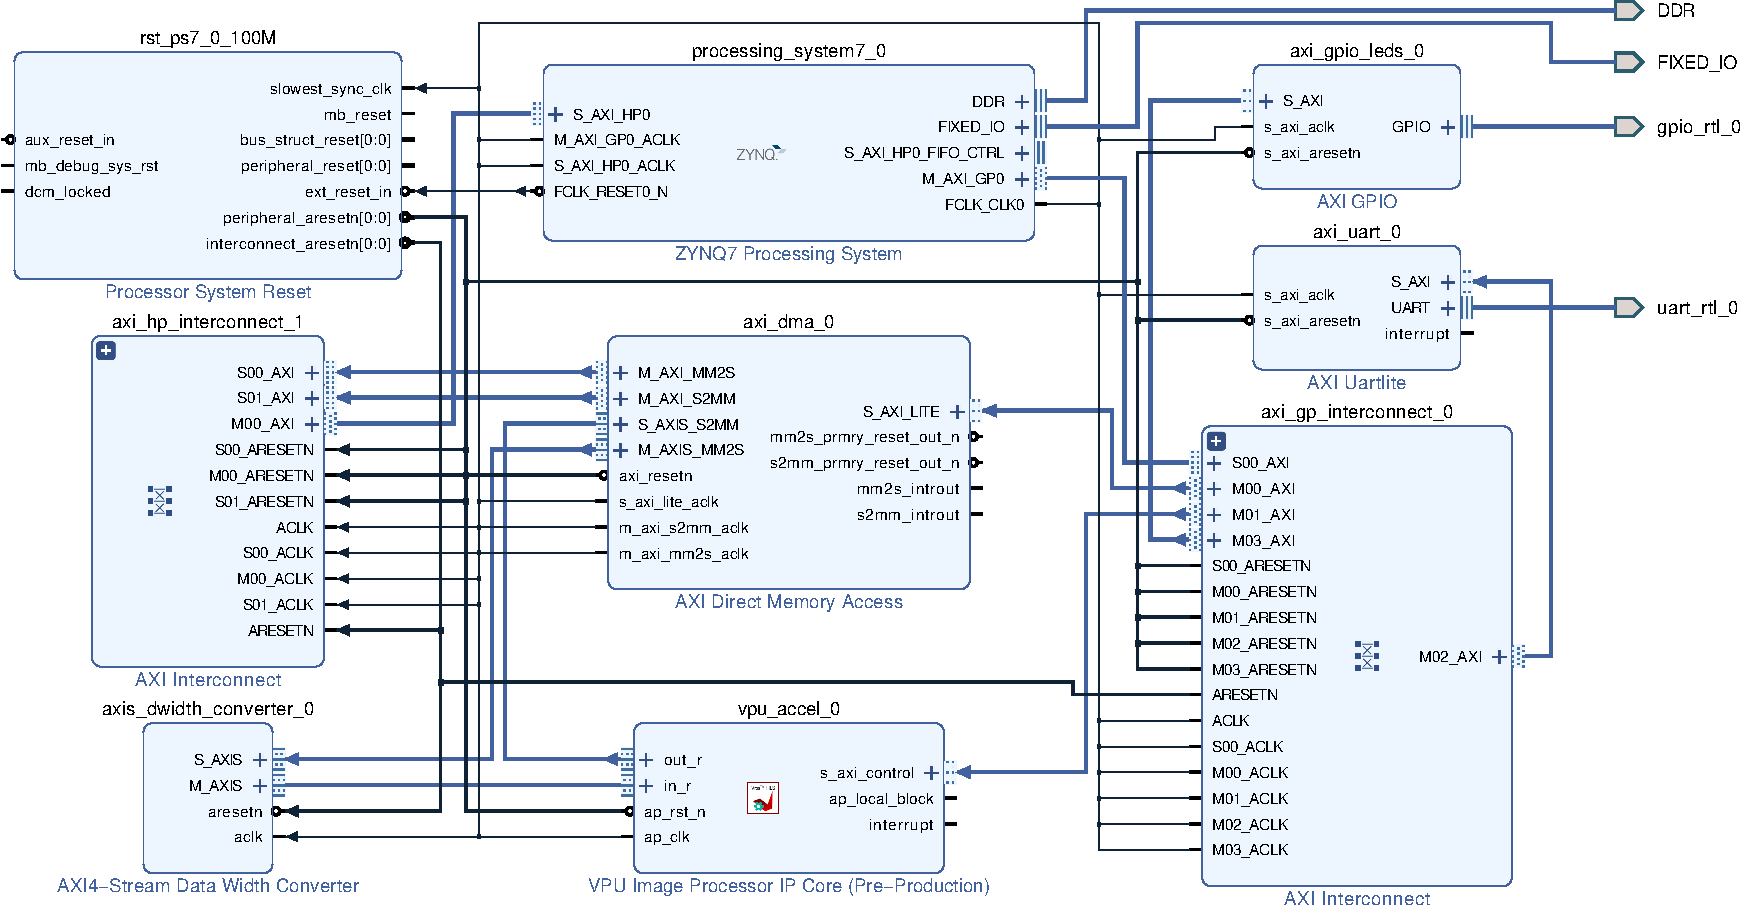
\includegraphics[angle=90, origin=c, clip, trim=0 0 16.60cm 0, width=1.25\textwidth]{hw-block-diagram-v2-crop-asset.pdf}}

			\end{paragraaf}
		\end{hoofdstuk}
	\end{appendices}

	% Empty last page
	\clearpage
	\thispagestyle{empty}
	\addtocounter{page}{-1}
	\ThisULCornerWallPaper{1.005}{asset_bg_last_page.jpg}
	\
	\clearpage

\end{document}
